\begin{figure}
\centering
%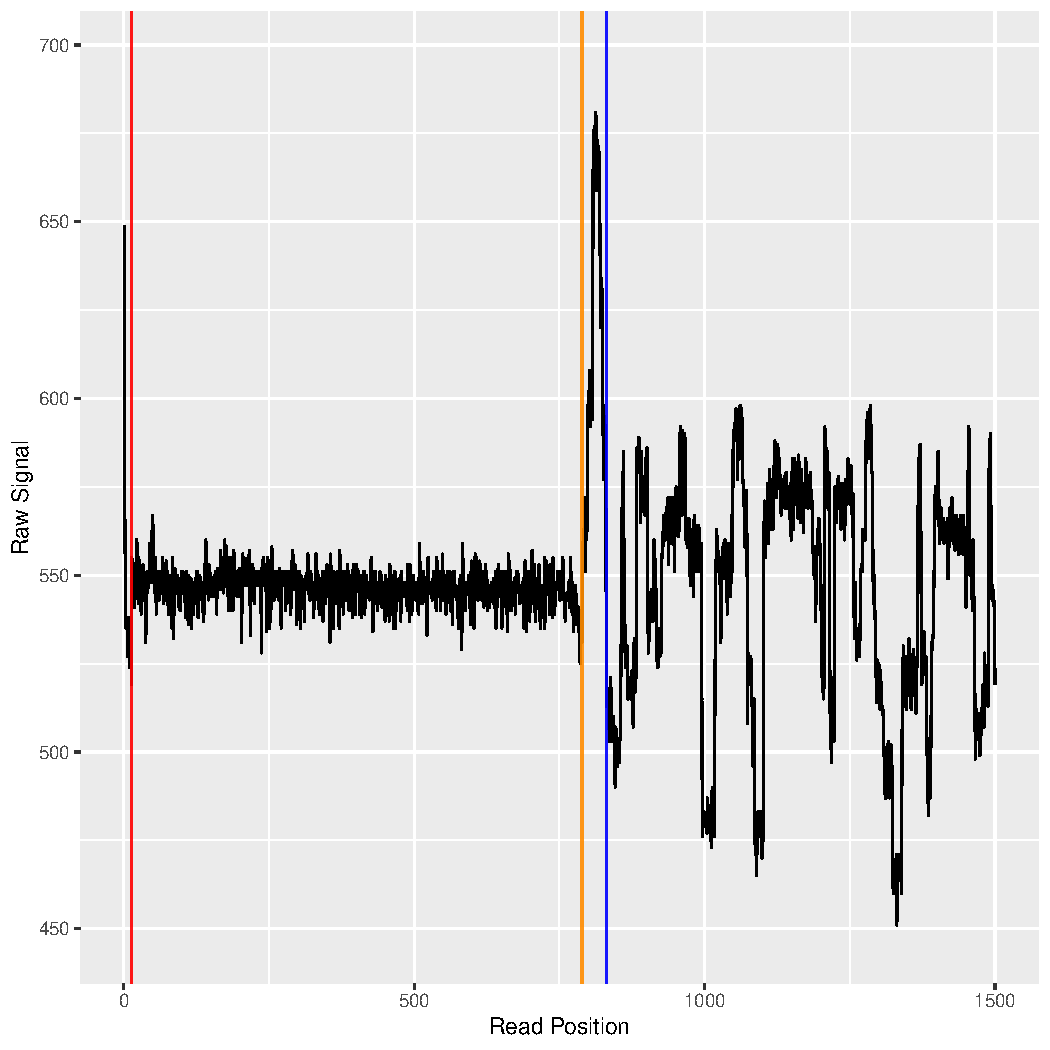
\includegraphics[scale=0.7]{evaluation/plots/reads.e9f08690-171f-476f-9119-5330d0290126.raw.section.pdf}
% Created by tikzDevice version 0.12.3.1 on 2022-09-20 16:09:06
% !TEX encoding = UTF-8 Unicode
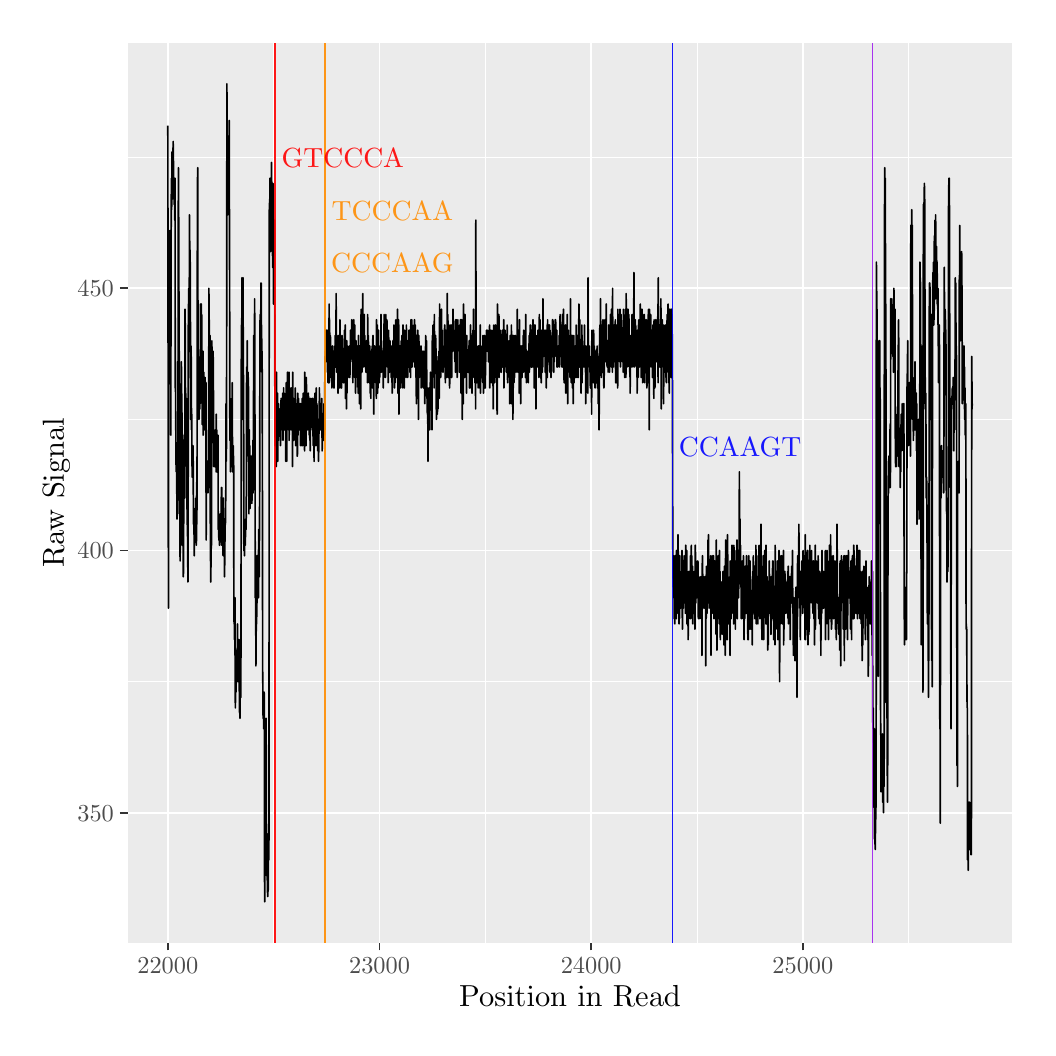
\begin{tikzpicture}[x=1pt,y=1pt]
\definecolor{fillColor}{RGB}{255,255,255}
\path[use as bounding box,fill=fillColor,fill opacity=0.00] (0,0) rectangle (361.35,361.35);
\begin{scope}
\path[clip] (  0.00,  0.00) rectangle (361.35,361.35);
\definecolor{drawColor}{RGB}{255,255,255}
\definecolor{fillColor}{RGB}{255,255,255}

\path[draw=drawColor,line width= 0.6pt,line join=round,line cap=round,fill=fillColor] (  0.00,  0.00) rectangle (361.35,361.35);
\end{scope}
\begin{scope}
\path[clip] ( 36.11, 30.69) rectangle (355.85,355.85);
\definecolor{fillColor}{gray}{0.92}

\path[fill=fillColor] ( 36.11, 30.69) rectangle (355.85,355.85);
\definecolor{drawColor}{RGB}{255,255,255}

\path[draw=drawColor,line width= 0.3pt,line join=round] ( 36.11,125.05) --
	(355.85,125.05);

\path[draw=drawColor,line width= 0.3pt,line join=round] ( 36.11,219.80) --
	(355.85,219.80);

\path[draw=drawColor,line width= 0.3pt,line join=round] ( 36.11,314.54) --
	(355.85,314.54);

\path[draw=drawColor,line width= 0.3pt,line join=round] ( 88.89, 30.69) --
	( 88.89,355.85);

\path[draw=drawColor,line width= 0.3pt,line join=round] (165.38, 30.69) --
	(165.38,355.85);

\path[draw=drawColor,line width= 0.3pt,line join=round] (241.88, 30.69) --
	(241.88,355.85);

\path[draw=drawColor,line width= 0.3pt,line join=round] (318.37, 30.69) --
	(318.37,355.85);

\path[draw=drawColor,line width= 0.6pt,line join=round] ( 36.11, 77.68) --
	(355.85, 77.68);

\path[draw=drawColor,line width= 0.6pt,line join=round] ( 36.11,172.42) --
	(355.85,172.42);

\path[draw=drawColor,line width= 0.6pt,line join=round] ( 36.11,267.17) --
	(355.85,267.17);

\path[draw=drawColor,line width= 0.6pt,line join=round] ( 50.64, 30.69) --
	( 50.64,355.85);

\path[draw=drawColor,line width= 0.6pt,line join=round] (127.14, 30.69) --
	(127.14,355.85);

\path[draw=drawColor,line width= 0.6pt,line join=round] (203.63, 30.69) --
	(203.63,355.85);

\path[draw=drawColor,line width= 0.6pt,line join=round] (280.12, 30.69) --
	(280.12,355.85);
\definecolor{drawColor}{RGB}{0,0,0}

\path[draw=drawColor,line width= 0.6pt,line join=round] ( 50.64,325.91) --
	( 50.72,261.48) --
	( 50.80,185.69) --
	( 50.87,151.58) --
	( 50.95,234.96) --
	( 51.03,272.85) --
	( 51.10,288.01) --
	( 51.18,269.06) --
	( 51.26,280.43) --
	( 51.33,250.11) --
	( 51.41,265.27) --
	( 51.49,284.22) --
	( 51.56,288.01) --
	( 51.64,231.17) --
	( 51.72,214.11) --
	( 51.79,269.06) --
	( 51.87,295.59) --
	( 51.95,306.96) --
	( 52.02,295.59) --
	( 52.10,303.17) --
	( 52.17,316.44) --
	( 52.25,299.38) --
	( 52.33,299.38) --
	( 52.40,314.54) --
	( 52.48,310.75) --
	( 52.56,320.23) --
	( 52.63,316.44) --
	( 52.71,308.86) --
	( 52.79,305.07) --
	( 52.86,305.07) --
	( 52.94,297.49) --
	( 53.02,303.17) --
	( 53.09,297.49) --
	( 53.17,291.80) --
	( 53.25,306.96) --
	( 53.32,231.17) --
	( 53.40,240.64) --
	( 53.47,223.59) --
	( 53.55,214.11) --
	( 53.63,202.74) --
	( 53.70,200.85) --
	( 53.78,202.74) --
	( 53.86,202.74) --
	( 53.93,183.79) --
	( 54.01,197.06) --
	( 54.09,185.69) --
	( 54.16,202.74) --
	( 54.24,208.43) --
	( 54.32,214.11) --
	( 54.39,280.43) --
	( 54.47,310.75) --
	( 54.55,297.49) --
	( 54.62,269.06) --
	( 54.70,261.48) --
	( 54.78,229.27) --
	( 54.85,185.69) --
	( 54.93,193.27) --
	( 55.00,181.90) --
	( 55.08,168.63) --
	( 55.16,178.11) --
	( 55.23,189.48) --
	( 55.31,202.74) --
	( 55.39,204.64) --
	( 55.46,204.64) --
	( 55.54,240.64) --
	( 55.62,231.17) --
	( 55.69,225.48) --
	( 55.77,219.80) --
	( 55.85,174.32) --
	( 55.92,197.06) --
	( 56.00,214.11) --
	( 56.08,195.16) --
	( 56.15,197.06) --
	( 56.23,162.95) --
	( 56.31,164.84) --
	( 56.38,185.69) --
	( 56.46,204.64) --
	( 56.53,200.85) --
	( 56.61,208.43) --
	( 56.69,208.43) --
	( 56.76,191.37) --
	( 56.84,259.59) --
	( 56.92,253.90) --
	( 56.99,227.38) --
	( 57.07,231.17) --
	( 57.15,223.59) --
	( 57.22,227.38) --
	( 57.30,216.01) --
	( 57.38,227.38) --
	( 57.45,214.11) --
	( 57.53,198.95) --
	( 57.61,185.69) --
	( 57.68,181.90) --
	( 57.76,180.00) --
	( 57.84,170.53) --
	( 57.91,161.05) --
	( 57.99,195.16) --
	( 58.06,261.48) --
	( 58.14,248.22) --
	( 58.22,267.17) --
	( 58.29,267.17) --
	( 58.37,244.43) --
	( 58.45,293.70) --
	( 58.52,276.64) --
	( 58.60,284.22) --
	( 58.68,274.75) --
	( 58.75,276.64) --
	( 58.83,246.32) --
	( 58.91,219.80) --
	( 58.98,236.85) --
	( 59.06,246.32) --
	( 59.14,229.27) --
	( 59.21,216.01) --
	( 59.29,221.69) --
	( 59.36,208.43) --
	( 59.44,198.95) --
	( 59.52,206.53) --
	( 59.59,200.85) --
	( 59.67,200.85) --
	( 59.75,210.32) --
	( 59.82,202.74) --
	( 59.90,181.90) --
	( 59.98,185.69) --
	( 60.05,183.79) --
	( 60.13,178.11) --
	( 60.21,170.53) --
	( 60.28,178.11) --
	( 60.36,183.79) --
	( 60.44,187.58) --
	( 60.51,183.79) --
	( 60.59,181.90) --
	( 60.67,180.00) --
	( 60.74,191.37) --
	( 60.82,183.79) --
	( 60.89,181.90) --
	( 60.97,174.32) --
	( 61.05,197.06) --
	( 61.12,181.90) --
	( 61.20,193.27) --
	( 61.28,269.06) --
	( 61.35,303.17) --
	( 61.43,310.75) --
	( 61.51,267.17) --
	( 61.58,225.48) --
	( 61.66,242.54) --
	( 61.74,223.59) --
	( 61.81,223.59) --
	( 61.89,219.80) --
	( 61.97,227.38) --
	( 62.04,225.48) --
	( 62.12,225.48) --
	( 62.20,223.59) --
	( 62.27,234.96) --
	( 62.35,225.48) --
	( 62.42,261.48) --
	( 62.50,236.85) --
	( 62.58,250.11) --
	( 62.65,244.43) --
	( 62.73,261.48) --
	( 62.81,242.54) --
	( 62.88,257.69) --
	( 62.96,242.54) --
	( 63.04,236.85) --
	( 63.11,217.90) --
	( 63.19,234.96) --
	( 63.27,231.17) --
	( 63.34,244.43) --
	( 63.42,214.11) --
	( 63.50,231.17) --
	( 63.57,216.01) --
	( 63.65,236.85) --
	( 63.72,221.69) --
	( 63.80,219.80) --
	( 63.88,216.01) --
	( 63.95,221.69) --
	( 64.03,217.90) --
	( 64.11,234.96) --
	( 64.18,231.17) --
	( 64.26,223.59) --
	( 64.34,229.27) --
	( 64.41,233.06) --
	( 64.49,176.21) --
	( 64.57,193.27) --
	( 64.64,200.85) --
	( 64.72,193.27) --
	( 64.80,204.64) --
	( 64.87,204.64) --
	( 64.95,195.16) --
	( 65.03,197.06) --
	( 65.10,197.06) --
	( 65.18,193.27) --
	( 65.25,198.95) --
	( 65.33,216.01) --
	( 65.41,195.16) --
	( 65.48,267.17) --
	( 65.56,253.90) --
	( 65.64,255.80) --
	( 65.71,233.06) --
	( 65.79,246.32) --
	( 65.87,250.11) --
	( 65.94,227.38) --
	( 66.02,168.63) --
	( 66.10,174.32) --
	( 66.17,161.05) --
	( 66.25,170.53) --
	( 66.33,174.32) --
	( 66.40,174.32) --
	( 66.48,208.43) --
	( 66.56,248.22) --
	( 66.63,238.75) --
	( 66.71,221.69) --
	( 66.78,233.06) --
	( 66.86,231.17) --
	( 66.94,238.75) --
	( 67.01,244.43) --
	( 67.09,234.96) --
	( 67.17,221.69) --
	( 67.24,202.74) --
	( 67.32,208.43) --
	( 67.40,206.53) --
	( 67.47,202.74) --
	( 67.55,208.43) --
	( 67.63,202.74) --
	( 67.70,212.22) --
	( 67.78,216.01) --
	( 67.86,208.43) --
	( 67.93,202.74) --
	( 68.01,212.22) --
	( 68.09,200.85) --
	( 68.16,221.69) --
	( 68.24,200.85) --
	( 68.31,216.01) --
	( 68.39,210.32) --
	( 68.47,200.85) --
	( 68.54,208.43) --
	( 68.62,202.74) --
	( 68.70,206.53) --
	( 68.77,214.11) --
	( 68.85,180.00) --
	( 68.93,183.79) --
	( 69.00,185.69) --
	( 69.08,176.21) --
	( 69.16,180.00) --
	( 69.23,178.11) --
	( 69.31,174.32) --
	( 69.39,181.90) --
	( 69.46,180.00) --
	( 69.54,178.11) --
	( 69.61,178.11) --
	( 69.69,185.69) --
	( 69.77,183.79) --
	( 69.84,180.00) --
	( 69.92,183.79) --
	( 70.00,195.16) --
	( 70.07,174.32) --
	( 70.15,195.16) --
	( 70.23,176.21) --
	( 70.30,189.48) --
	( 70.38,178.11) --
	( 70.46,185.69) --
	( 70.53,180.00) --
	( 70.61,170.53) --
	( 70.69,191.37) --
	( 70.76,172.42) --
	( 70.84,178.11) --
	( 70.92,176.21) --
	( 70.99,180.00) --
	( 71.07,183.79) --
	( 71.14,162.95) --
	( 71.22,170.53) --
	( 71.30,178.11) --
	( 71.37,181.90) --
	( 71.45,181.90) --
	( 71.53,189.48) --
	( 71.60,193.27) --
	( 71.68,225.48) --
	( 71.76,204.64) --
	( 71.83,210.32) --
	( 71.91,255.80) --
	( 71.99,341.07) --
	( 72.06,306.96) --
	( 72.14,301.28) --
	( 72.22,314.54) --
	( 72.29,293.70) --
	( 72.37,320.23) --
	( 72.45,322.12) --
	( 72.52,320.23) --
	( 72.60,318.33) --
	( 72.67,314.54) --
	( 72.75,303.17) --
	( 72.83,327.81) --
	( 72.90,295.59) --
	( 72.98,265.27) --
	( 73.06,212.22) --
	( 73.13,219.80) --
	( 73.21,227.38) --
	( 73.29,200.85) --
	( 73.36,221.69) --
	( 73.44,216.01) --
	( 73.52,212.22) --
	( 73.59,214.11) --
	( 73.67,202.74) --
	( 73.75,217.90) --
	( 73.82,221.69) --
	( 73.90,233.06) --
	( 73.97,216.01) --
	( 74.05,200.85) --
	( 74.13,210.32) --
	( 74.20,206.53) --
	( 74.28,210.32) --
	( 74.36,200.85) --
	( 74.43,206.53) --
	( 74.51,155.37) --
	( 74.59,145.90) --
	( 74.66,149.69) --
	( 74.74,140.21) --
	( 74.82,145.90) --
	( 74.89,155.37) --
	( 74.97,125.05) --
	( 75.05,115.58) --
	( 75.12,123.16) --
	( 75.20,136.42) --
	( 75.28,121.26) --
	( 75.35,125.05) --
	( 75.43,134.53) --
	( 75.50,125.05) --
	( 75.58,130.74) --
	( 75.66,130.74) --
	( 75.73,132.63) --
	( 75.81,145.90) --
	( 75.89,132.63) --
	( 75.96,140.21) --
	( 76.04,125.05) --
	( 76.12,130.74) --
	( 76.19,134.53) --
	( 76.27,140.21) --
	( 76.35,125.05) --
	( 76.42,140.21) --
	( 76.50,115.58) --
	( 76.58,113.68) --
	( 76.65,123.16) --
	( 76.73,111.79) --
	( 76.81,132.63) --
	( 76.88,125.05) --
	( 76.96,132.63) --
	( 77.03,119.37) --
	( 77.11,164.84) --
	( 77.19,238.75) --
	( 77.26,253.90) --
	( 77.34,238.75) --
	( 77.42,270.96) --
	( 77.49,259.59) --
	( 77.57,269.06) --
	( 77.65,233.06) --
	( 77.72,219.80) --
	( 77.80,270.96) --
	( 77.88,250.11) --
	( 77.95,236.85) --
	( 78.03,227.38) --
	( 78.11,172.42) --
	( 78.18,174.32) --
	( 78.26,181.90) --
	( 78.34,170.53) --
	( 78.41,180.00) --
	( 78.49,178.11) --
	( 78.56,178.11) --
	( 78.64,174.32) --
	( 78.72,180.00) --
	( 78.79,183.79) --
	( 78.87,180.00) --
	( 78.95,183.79) --
	( 79.02,193.27) --
	( 79.10,233.06) --
	( 79.18,238.75) --
	( 79.25,206.53) --
	( 79.33,248.22) --
	( 79.41,234.96) --
	( 79.48,233.06) --
	( 79.56,234.96) --
	( 79.64,236.85) --
	( 79.71,233.06) --
	( 79.79,231.17) --
	( 79.86,204.64) --
	( 79.94,185.69) --
	( 80.02,208.43) --
	( 80.09,216.01) --
	( 80.17,195.16) --
	( 80.25,210.32) --
	( 80.32,187.58) --
	( 80.40,204.64) --
	( 80.48,197.06) --
	( 80.55,191.37) --
	( 80.63,189.48) --
	( 80.71,206.53) --
	( 80.78,195.16) --
	( 80.86,197.06) --
	( 80.94,189.48) --
	( 81.01,189.48) --
	( 81.09,193.27) --
	( 81.17,202.74) --
	( 81.24,200.85) --
	( 81.32,200.85) --
	( 81.39,212.22) --
	( 81.47,193.27) --
	( 81.55,212.22) --
	( 81.62,227.38) --
	( 81.70,250.11) --
	( 81.78,242.54) --
	( 81.85,246.32) --
	( 81.93,240.64) --
	( 82.01,263.38) --
	( 82.08,236.85) --
	( 82.16,200.85) --
	( 82.24,155.37) --
	( 82.31,159.16) --
	( 82.39,162.95) --
	( 82.47,130.74) --
	( 82.54,138.32) --
	( 82.62,153.48) --
	( 82.70,145.90) --
	( 82.77,149.69) --
	( 82.85,170.53) --
	( 82.92,153.48) --
	( 83.00,170.53) --
	( 83.08,161.05) --
	( 83.15,168.63) --
	( 83.23,159.16) --
	( 83.31,164.84) --
	( 83.38,155.37) --
	( 83.46,180.00) --
	( 83.54,170.53) --
	( 83.61,168.63) --
	( 83.69,162.95) --
	( 83.77,183.79) --
	( 83.84,195.16) --
	( 83.92,250.11) --
	( 84.00,257.69) --
	( 84.07,240.64) --
	( 84.15,248.22) --
	( 84.22,253.90) --
	( 84.30,269.06) --
	( 84.38,269.06) --
	( 84.45,252.01) --
	( 84.53,253.90) --
	( 84.61,236.85) --
	( 84.68,244.43) --
	( 84.76,234.96) --
	( 84.84,183.79) --
	( 84.91,128.84) --
	( 84.99,123.16) --
	( 85.07,111.79) --
	( 85.14,121.26) --
	( 85.22,117.47) --
	( 85.30,108.00) --
	( 85.37,121.26) --
	( 85.45,121.26) --
	( 85.53,117.47) --
	( 85.60, 53.05) --
	( 85.68, 45.47) --
	( 85.75, 79.57) --
	( 85.83, 68.20) --
	( 85.91, 83.36) --
	( 85.98, 94.73) --
	( 86.06,108.00) --
	( 86.14,111.79) --
	( 86.21, 94.73) --
	( 86.29, 66.31) --
	( 86.37, 54.94) --
	( 86.44, 64.41) --
	( 86.52, 62.52) --
	( 86.60, 53.05) --
	( 86.67, 49.26) --
	( 86.75, 47.36) --
	( 86.83, 62.52) --
	( 86.90, 49.26) --
	( 86.98, 70.10) --
	( 87.06, 62.52) --
	( 87.13, 60.63) --
	( 87.21, 73.89) --
	( 87.28,295.59) --
	( 87.36,295.59) --
	( 87.44,299.38) --
	( 87.51,299.38) --
	( 87.59,306.96) --
	( 87.67,289.91) --
	( 87.74,280.43) --
	( 87.82,299.38) --
	( 87.90,295.59) --
	( 87.97,289.91) --
	( 88.05,291.80) --
	( 88.13,312.65) --
	( 88.20,299.38) --
	( 88.28,288.01) --
	( 88.36,288.01) --
	( 88.43,297.49) --
	( 88.51,274.75) --
	( 88.59,276.64) --
	( 88.66,305.07) --
	( 88.74,295.59) --
	( 88.81,261.48) --
	( 88.89,282.33) --
	( 88.97,282.33) --
	( 89.04,286.12) --
	( 89.12,278.54) --
	( 89.20,291.80) --
	( 89.27,244.43) --
	( 89.35,217.90) --
	( 89.43,210.32) --
	( 89.50,225.48) --
	( 89.58,210.32) --
	( 89.66,217.90) --
	( 89.73,221.69) --
	( 89.81,202.74) --
	( 89.89,236.85) --
	( 89.96,229.27) --
	( 90.04,223.59) --
	( 90.11,223.59) --
	( 90.19,227.38) --
	( 90.27,229.27) --
	( 90.34,204.64) --
	( 90.42,221.69) --
	( 90.50,214.11) --
	( 90.57,212.22) --
	( 90.65,225.48) --
	( 90.73,219.80) --
	( 90.80,216.01) --
	( 90.88,223.59) --
	( 90.96,223.59) --
	( 91.03,219.80) --
	( 91.11,217.90) --
	( 91.19,217.90) --
	( 91.26,216.01) --
	( 91.34,210.32) --
	( 91.42,212.22) --
	( 91.49,212.22) --
	( 91.57,227.38) --
	( 91.64,216.01) --
	( 91.72,219.80) --
	( 91.80,225.48) --
	( 91.87,221.69) --
	( 91.95,223.59) --
	( 92.03,219.80) --
	( 92.10,223.59) --
	( 92.18,229.27) --
	( 92.26,212.22) --
	( 92.33,223.59) --
	( 92.41,223.59) --
	( 92.49,231.17) --
	( 92.56,216.01) --
	( 92.64,216.01) --
	( 92.72,229.27) --
	( 92.79,225.48) --
	( 92.87,216.01) --
	( 92.95,225.48) --
	( 93.02,223.59) --
	( 93.10,227.38) --
	( 93.17,227.38) --
	( 93.25,204.64) --
	( 93.33,208.43) --
	( 93.40,233.06) --
	( 93.48,214.11) --
	( 93.56,216.01) --
	( 93.63,204.64) --
	( 93.71,231.17) --
	( 93.79,217.90) --
	( 93.86,236.85) --
	( 93.94,219.80) --
	( 94.02,231.17) --
	( 94.09,233.06) --
	( 94.17,223.59) --
	( 94.25,216.01) --
	( 94.32,229.27) --
	( 94.40,236.85) --
	( 94.47,212.22) --
	( 94.55,219.80) --
	( 94.63,216.01) --
	( 94.70,223.59) --
	( 94.78,231.17) --
	( 94.86,229.27) --
	( 94.93,217.90) --
	( 95.01,229.27) --
	( 95.09,217.90) --
	( 95.16,216.01) --
	( 95.24,223.59) --
	( 95.32,231.17) --
	( 95.39,221.69) --
	( 95.47,216.01) --
	( 95.55,223.59) --
	( 95.62,219.80) --
	( 95.70,202.74) --
	( 95.78,236.85) --
	( 95.85,214.11) --
	( 95.93,219.80) --
	( 96.00,225.48) --
	( 96.08,227.38) --
	( 96.16,212.22) --
	( 96.23,223.59) --
	( 96.31,219.80) --
	( 96.39,225.48) --
	( 96.46,219.80) --
	( 96.54,216.01) --
	( 96.62,225.48) --
	( 96.69,231.17) --
	( 96.77,225.48) --
	( 96.85,210.32) --
	( 96.92,219.80) --
	( 97.00,216.01) --
	( 97.08,216.01) --
	( 97.15,216.01) --
	( 97.23,216.01) --
	( 97.31,225.48) --
	( 97.38,206.53) --
	( 97.46,206.53) --
	( 97.53,210.32) --
	( 97.61,229.27) --
	( 97.69,214.11) --
	( 97.76,219.80) --
	( 97.84,227.38) --
	( 97.92,219.80) --
	( 97.99,225.48) --
	( 98.07,216.01) --
	( 98.15,223.59) --
	( 98.22,216.01) --
	( 98.30,223.59) --
	( 98.38,219.80) --
	( 98.45,225.48) --
	( 98.53,223.59) --
	( 98.61,210.32) --
	( 98.68,225.48) --
	( 98.76,212.22) --
	( 98.84,217.90) --
	( 98.91,221.69) --
	( 98.99,219.80) --
	( 99.06,210.32) --
	( 99.14,223.59) --
	( 99.22,227.38) --
	( 99.29,221.69) --
	( 99.37,210.32) --
	( 99.45,219.80) --
	( 99.52,219.80) --
	( 99.60,229.27) --
	( 99.68,221.69) --
	( 99.75,221.69) --
	( 99.83,216.01) --
	( 99.91,221.69) --
	( 99.98,227.38) --
	(100.06,208.43) --
	(100.14,236.85) --
	(100.21,216.01) --
	(100.29,216.01) --
	(100.36,219.80) --
	(100.44,210.32) --
	(100.52,216.01) --
	(100.59,210.32) --
	(100.67,234.96) --
	(100.75,231.17) --
	(100.82,229.27) --
	(100.90,227.38) --
	(100.98,217.90) --
	(101.05,221.69) --
	(101.13,216.01) --
	(101.21,223.59) --
	(101.28,227.38) --
	(101.36,225.48) --
	(101.44,229.27) --
	(101.51,216.01) --
	(101.59,223.59) --
	(101.67,221.69) --
	(101.74,214.11) --
	(101.82,227.38) --
	(101.89,216.01) --
	(101.97,212.22) --
	(102.05,214.11) --
	(102.12,208.43) --
	(102.20,227.38) --
	(102.28,217.90) --
	(102.35,223.59) --
	(102.43,221.69) --
	(102.51,219.80) --
	(102.58,221.69) --
	(102.66,225.48) --
	(102.74,227.38) --
	(102.81,217.90) --
	(102.89,216.01) --
	(102.97,227.38) --
	(103.04,219.80) --
	(103.12,214.11) --
	(103.20,210.32) --
	(103.27,210.32) --
	(103.35,217.90) --
	(103.42,216.01) --
	(103.50,204.64) --
	(103.58,221.69) --
	(103.65,227.38) --
	(103.73,227.38) --
	(103.81,229.27) --
	(103.88,216.01) --
	(103.96,214.11) --
	(104.04,225.48) --
	(104.11,221.69) --
	(104.19,210.32) --
	(104.27,231.17) --
	(104.34,223.59) --
	(104.42,223.59) --
	(104.50,225.48) --
	(104.57,223.59) --
	(104.65,216.01) --
	(104.72,219.80) --
	(104.80,208.43) --
	(104.88,210.32) --
	(104.95,219.80) --
	(105.03,212.22) --
	(105.11,204.64) --
	(105.18,210.32) --
	(105.26,216.01) --
	(105.34,216.01) --
	(105.41,231.17) --
	(105.49,216.01) --
	(105.57,225.48) --
	(105.64,216.01) --
	(105.72,223.59) --
	(105.80,225.48) --
	(105.87,221.69) --
	(105.95,216.01) --
	(106.03,223.59) --
	(106.10,219.80) --
	(106.18,223.59) --
	(106.25,227.38) --
	(106.33,221.69) --
	(106.41,208.43) --
	(106.48,217.90) --
	(106.56,219.80) --
	(106.64,221.69) --
	(106.71,212.22) --
	(106.79,214.11) --
	(106.87,214.11) --
	(106.94,214.11) --
	(107.02,212.22) --
	(107.10,225.48) --
	(107.17,214.11) --
	(107.25,221.69) --
	(107.33,216.01) --
	(107.40,242.54) --
	(107.48,240.64) --
	(107.56,240.64) --
	(107.63,244.43) --
	(107.71,240.64) --
	(107.78,252.01) --
	(107.86,246.32) --
	(107.94,246.32) --
	(108.01,242.54) --
	(108.09,252.01) --
	(108.17,240.64) --
	(108.24,252.01) --
	(108.32,236.85) --
	(108.40,238.75) --
	(108.47,250.11) --
	(108.55,233.06) --
	(108.63,240.64) --
	(108.70,233.06) --
	(108.78,238.75) --
	(108.86,242.54) --
	(108.93,261.48) --
	(109.01,233.06) --
	(109.09,255.80) --
	(109.16,246.32) --
	(109.24,250.11) --
	(109.31,238.75) --
	(109.39,250.11) --
	(109.47,242.54) --
	(109.54,234.96) --
	(109.62,240.64) --
	(109.70,236.85) --
	(109.77,242.54) --
	(109.85,238.75) --
	(109.93,231.17) --
	(110.00,233.06) --
	(110.08,242.54) --
	(110.16,246.32) --
	(110.23,238.75) --
	(110.31,238.75) --
	(110.39,240.64) --
	(110.46,233.06) --
	(110.54,234.96) --
	(110.61,244.43) --
	(110.69,231.17) --
	(110.77,234.96) --
	(110.84,238.75) --
	(110.92,246.32) --
	(111.00,246.32) --
	(111.07,238.75) --
	(111.15,250.11) --
	(111.23,238.75) --
	(111.30,246.32) --
	(111.38,240.64) --
	(111.46,265.27) --
	(111.53,240.64) --
	(111.61,238.75) --
	(111.69,236.85) --
	(111.76,246.32) --
	(111.84,242.54) --
	(111.92,238.75) --
	(111.99,242.54) --
	(112.07,240.64) --
	(112.14,229.27) --
	(112.22,250.11) --
	(112.30,242.54) --
	(112.37,244.43) --
	(112.45,242.54) --
	(112.53,236.85) --
	(112.60,231.17) --
	(112.68,250.11) --
	(112.76,242.54) --
	(112.83,255.80) --
	(112.91,240.64) --
	(112.99,246.32) --
	(113.06,244.43) --
	(113.14,234.96) --
	(113.22,231.17) --
	(113.29,236.85) --
	(113.37,244.43) --
	(113.45,231.17) --
	(113.52,250.11) --
	(113.60,250.11) --
	(113.67,242.54) --
	(113.75,244.43) --
	(113.83,234.96) --
	(113.90,238.75) --
	(113.98,236.85) --
	(114.06,233.06) --
	(114.13,236.85) --
	(114.21,240.64) --
	(114.29,233.06) --
	(114.36,238.75) --
	(114.44,252.01) --
	(114.52,244.43) --
	(114.59,244.43) --
	(114.67,242.54) --
	(114.75,253.90) --
	(114.82,227.38) --
	(114.90,240.64) --
	(114.97,246.32) --
	(115.05,248.22) --
	(115.13,234.96) --
	(115.20,223.59) --
	(115.28,248.22) --
	(115.36,229.27) --
	(115.43,240.64) --
	(115.51,240.64) --
	(115.59,246.32) --
	(115.66,236.85) --
	(115.74,234.96) --
	(115.82,240.64) --
	(115.89,240.64) --
	(115.97,242.54) --
	(116.05,236.85) --
	(116.12,238.75) --
	(116.20,240.64) --
	(116.28,246.32) --
	(116.35,234.96) --
	(116.43,234.96) --
	(116.50,240.64) --
	(116.58,242.54) --
	(116.66,252.01) --
	(116.73,246.32) --
	(116.81,248.22) --
	(116.89,248.22) --
	(116.96,246.32) --
	(117.04,244.43) --
	(117.12,255.80) --
	(117.19,242.54) --
	(117.27,240.64) --
	(117.35,244.43) --
	(117.42,250.11) --
	(117.50,233.06) --
	(117.58,248.22) --
	(117.65,244.43) --
	(117.73,242.54) --
	(117.81,255.80) --
	(117.88,240.64) --
	(117.96,240.64) --
	(118.03,246.32) --
	(118.11,234.96) --
	(118.19,253.90) --
	(118.26,238.75) --
	(118.34,240.64) --
	(118.42,234.96) --
	(118.49,229.27) --
	(118.57,234.96) --
	(118.65,248.22) --
	(118.72,244.43) --
	(118.80,236.85) --
	(118.88,246.32) --
	(118.95,240.64) --
	(119.03,246.32) --
	(119.11,234.96) --
	(119.18,238.75) --
	(119.26,242.54) --
	(119.34,236.85) --
	(119.41,229.27) --
	(119.49,246.32) --
	(119.56,250.11) --
	(119.64,236.85) --
	(119.72,242.54) --
	(119.79,242.54) --
	(119.87,225.48) --
	(119.95,238.75) --
	(120.02,246.32) --
	(120.10,238.75) --
	(120.18,242.54) --
	(120.25,236.85) --
	(120.33,223.59) --
	(120.41,236.85) --
	(120.48,259.59) --
	(120.56,242.54) --
	(120.64,246.32) --
	(120.71,242.54) --
	(120.79,236.85) --
	(120.86,242.54) --
	(120.94,246.32) --
	(121.02,255.80) --
	(121.09,265.27) --
	(121.17,252.01) --
	(121.25,252.01) --
	(121.32,238.75) --
	(121.40,246.32) --
	(121.48,250.11) --
	(121.55,240.64) --
	(121.63,257.69) --
	(121.71,244.43) --
	(121.78,250.11) --
	(121.86,246.32) --
	(121.94,238.75) --
	(122.01,238.75) --
	(122.09,244.43) --
	(122.17,238.75) --
	(122.24,236.85) --
	(122.32,242.54) --
	(122.39,248.22) --
	(122.47,248.22) --
	(122.55,244.43) --
	(122.62,242.54) --
	(122.70,242.54) --
	(122.78,233.06) --
	(122.85,257.69) --
	(122.93,242.54) --
	(123.01,234.96) --
	(123.08,250.11) --
	(123.16,246.32) --
	(123.24,240.64) --
	(123.31,242.54) --
	(123.39,233.06) --
	(123.47,236.85) --
	(123.54,234.96) --
	(123.62,246.32) --
	(123.70,242.54) --
	(123.77,229.27) --
	(123.85,244.43) --
	(123.92,244.43) --
	(124.00,227.38) --
	(124.08,238.75) --
	(124.15,231.17) --
	(124.23,238.75) --
	(124.31,236.85) --
	(124.38,238.75) --
	(124.46,246.32) --
	(124.54,238.75) --
	(124.61,231.17) --
	(124.69,248.22) --
	(124.77,250.11) --
	(124.84,233.06) --
	(124.92,233.06) --
	(125.00,236.85) --
	(125.07,221.69) --
	(125.15,246.32) --
	(125.22,242.54) --
	(125.30,244.43) --
	(125.38,246.32) --
	(125.45,236.85) --
	(125.53,240.64) --
	(125.61,238.75) --
	(125.68,242.54) --
	(125.76,233.06) --
	(125.84,240.64) --
	(125.91,238.75) --
	(125.99,227.38) --
	(126.07,255.80) --
	(126.14,238.75) --
	(126.22,238.75) --
	(126.30,236.85) --
	(126.37,253.90) --
	(126.45,229.27) --
	(126.53,246.32) --
	(126.60,231.17) --
	(126.68,244.43) --
	(126.75,252.01) --
	(126.83,244.43) --
	(126.91,234.96) --
	(126.98,242.54) --
	(127.06,233.06) --
	(127.14,244.43) --
	(127.21,234.96) --
	(127.29,242.54) --
	(127.37,246.32) --
	(127.44,238.75) --
	(127.52,236.85) --
	(127.60,238.75) --
	(127.67,257.69) --
	(127.75,242.54) --
	(127.83,236.85) --
	(127.90,244.43) --
	(127.98,238.75) --
	(128.06,240.64) --
	(128.13,238.75) --
	(128.21,244.43) --
	(128.28,236.85) --
	(128.36,238.75) --
	(128.44,240.64) --
	(128.51,231.17) --
	(128.59,248.22) --
	(128.67,234.96) --
	(128.74,250.11) --
	(128.82,257.69) --
	(128.90,242.54) --
	(128.97,248.22) --
	(129.05,246.32) --
	(129.13,238.75) --
	(129.20,236.85) --
	(129.28,234.96) --
	(129.36,244.43) --
	(129.43,257.69) --
	(129.51,246.32) --
	(129.59,248.22) --
	(129.66,250.11) --
	(129.74,246.32) --
	(129.81,255.80) --
	(129.89,240.64) --
	(129.97,238.75) --
	(130.04,240.64) --
	(130.12,240.64) --
	(130.20,248.22) --
	(130.27,233.06) --
	(130.35,242.54) --
	(130.43,252.01) --
	(130.50,238.75) --
	(130.58,240.64) --
	(130.66,238.75) --
	(130.73,236.85) --
	(130.81,242.54) --
	(130.89,248.22) --
	(130.96,246.32) --
	(131.04,238.75) --
	(131.11,246.32) --
	(131.19,240.64) --
	(131.27,240.64) --
	(131.34,234.96) --
	(131.42,238.75) --
	(131.50,246.32) --
	(131.57,236.85) --
	(131.65,234.96) --
	(131.73,229.27) --
	(131.80,238.75) --
	(131.88,234.96) --
	(131.96,248.22) --
	(132.03,244.43) --
	(132.11,246.32) --
	(132.19,242.54) --
	(132.26,240.64) --
	(132.34,253.90) --
	(132.42,242.54) --
	(132.49,242.54) --
	(132.57,231.17) --
	(132.64,240.64) --
	(132.72,246.32) --
	(132.80,233.06) --
	(132.87,244.43) --
	(132.95,246.32) --
	(133.03,255.80) --
	(133.10,240.64) --
	(133.18,234.96) --
	(133.26,238.75) --
	(133.33,236.85) --
	(133.41,244.43) --
	(133.49,250.11) --
	(133.56,238.75) --
	(133.64,259.59) --
	(133.72,250.11) --
	(133.79,229.27) --
	(133.87,248.22) --
	(133.95,231.17) --
	(134.02,255.80) --
	(134.10,252.01) --
	(134.17,221.69) --
	(134.25,246.32) --
	(134.33,236.85) --
	(134.40,242.54) --
	(134.48,238.75) --
	(134.56,246.32) --
	(134.63,246.32) --
	(134.71,231.17) --
	(134.79,233.06) --
	(134.86,244.43) --
	(134.94,242.54) --
	(135.02,248.22) --
	(135.09,246.32) --
	(135.17,244.43) --
	(135.25,250.11) --
	(135.32,244.43) --
	(135.40,250.11) --
	(135.47,242.54) --
	(135.55,231.17) --
	(135.63,253.90) --
	(135.70,250.11) --
	(135.78,248.22) --
	(135.86,238.75) --
	(135.93,248.22) --
	(136.01,238.75) --
	(136.09,231.17) --
	(136.16,252.01) --
	(136.24,240.64) --
	(136.32,236.85) --
	(136.39,246.32) --
	(136.47,246.32) --
	(136.55,238.75) --
	(136.62,246.32) --
	(136.70,248.22) --
	(136.78,234.96) --
	(136.85,253.90) --
	(136.93,240.64) --
	(137.00,238.75) --
	(137.08,238.75) --
	(137.16,240.64) --
	(137.23,248.22) --
	(137.31,234.96) --
	(137.39,244.43) --
	(137.46,240.64) --
	(137.54,248.22) --
	(137.62,238.75) --
	(137.69,238.75) --
	(137.77,252.01) --
	(137.85,240.64) --
	(137.92,242.54) --
	(138.00,244.43) --
	(138.08,252.01) --
	(138.15,236.85) --
	(138.23,244.43) --
	(138.31,246.32) --
	(138.38,234.96) --
	(138.46,255.80) --
	(138.53,250.11) --
	(138.61,252.01) --
	(138.69,238.75) --
	(138.76,255.80) --
	(138.84,238.75) --
	(138.92,238.75) --
	(138.99,250.11) --
	(139.07,240.64) --
	(139.15,240.64) --
	(139.22,250.11) --
	(139.30,246.32) --
	(139.38,240.64) --
	(139.45,244.43) --
	(139.53,253.90) --
	(139.61,242.54) --
	(139.68,248.22) --
	(139.76,255.80) --
	(139.84,238.75) --
	(139.91,244.43) --
	(139.99,252.01) --
	(140.06,253.90) --
	(140.14,240.64) --
	(140.22,246.32) --
	(140.29,234.96) --
	(140.37,244.43) --
	(140.45,225.48) --
	(140.52,250.11) --
	(140.60,240.64) --
	(140.68,233.06) --
	(140.75,233.06) --
	(140.83,227.38) --
	(140.91,252.01) --
	(140.98,252.01) --
	(141.06,246.32) --
	(141.14,234.96) --
	(141.21,219.80) --
	(141.29,250.11) --
	(141.36,250.11) --
	(141.44,238.75) --
	(141.52,234.96) --
	(141.59,240.64) --
	(141.67,242.54) --
	(141.75,236.85) --
	(141.82,244.43) --
	(141.90,240.64) --
	(141.98,242.54) --
	(142.05,238.75) --
	(142.13,246.32) --
	(142.21,231.17) --
	(142.28,238.75) --
	(142.36,236.85) --
	(142.44,240.64) --
	(142.51,244.43) --
	(142.59,244.43) --
	(142.67,236.85) --
	(142.74,240.64) --
	(142.82,234.96) --
	(142.89,240.64) --
	(142.97,231.17) --
	(143.05,242.54) --
	(143.12,244.43) --
	(143.20,236.85) --
	(143.28,242.54) --
	(143.35,238.75) --
	(143.43,234.96) --
	(143.51,225.48) --
	(143.58,231.17) --
	(143.66,244.43) --
	(143.74,240.64) --
	(143.81,250.11) --
	(143.89,244.43) --
	(143.97,242.54) --
	(144.04,246.32) --
	(144.12,248.22) --
	(144.20,233.06) --
	(144.27,227.38) --
	(144.35,227.38) --
	(144.42,221.69) --
	(144.50,231.17) --
	(144.58,221.69) --
	(144.65,204.64) --
	(144.73,229.27) --
	(144.81,216.01) --
	(144.88,223.59) --
	(144.96,227.38) --
	(145.04,231.17) --
	(145.11,223.59) --
	(145.19,229.27) --
	(145.27,216.01) --
	(145.34,221.69) --
	(145.42,233.06) --
	(145.50,225.48) --
	(145.57,236.85) --
	(145.65,229.27) --
	(145.72,233.06) --
	(145.80,229.27) --
	(145.88,225.48) --
	(145.95,231.17) --
	(146.03,233.06) --
	(146.11,216.01) --
	(146.18,246.32) --
	(146.26,250.11) --
	(146.34,236.85) --
	(146.41,238.75) --
	(146.49,253.90) --
	(146.57,242.54) --
	(146.64,246.32) --
	(146.72,242.54) --
	(146.80,246.32) --
	(146.87,231.17) --
	(146.95,257.69) --
	(147.03,238.75) --
	(147.10,244.43) --
	(147.18,240.64) --
	(147.25,248.22) --
	(147.33,242.54) --
	(147.41,250.11) --
	(147.48,246.32) --
	(147.56,244.43) --
	(147.64,225.48) --
	(147.71,219.80) --
	(147.79,242.54) --
	(147.87,229.27) --
	(147.94,231.17) --
	(148.02,221.69) --
	(148.10,223.59) --
	(148.17,225.48) --
	(148.25,223.59) --
	(148.33,227.38) --
	(148.40,229.27) --
	(148.48,233.06) --
	(148.56,240.64) --
	(148.63,244.43) --
	(148.71,227.38) --
	(148.78,242.54) --
	(148.86,261.48) --
	(148.94,240.64) --
	(149.01,252.01) --
	(149.09,240.64) --
	(149.17,246.32) --
	(149.24,234.96) --
	(149.32,250.11) --
	(149.40,248.22) --
	(149.47,244.43) --
	(149.55,259.59) --
	(149.63,246.32) --
	(149.70,242.54) --
	(149.78,252.01) --
	(149.86,244.43) --
	(149.93,246.32) --
	(150.01,236.85) --
	(150.09,236.85) --
	(150.16,240.64) --
	(150.24,244.43) --
	(150.31,238.75) --
	(150.39,238.75) --
	(150.47,246.32) --
	(150.54,244.43) --
	(150.62,252.01) --
	(150.70,253.90) --
	(150.77,252.01) --
	(150.85,240.64) --
	(150.93,233.06) --
	(151.00,238.75) --
	(151.08,252.01) --
	(151.16,244.43) --
	(151.23,244.43) --
	(151.31,244.43) --
	(151.39,240.64) --
	(151.46,234.96) --
	(151.54,240.64) --
	(151.61,265.27) --
	(151.69,242.54) --
	(151.77,242.54) --
	(151.84,257.69) --
	(151.92,244.43) --
	(152.00,234.96) --
	(152.07,246.32) --
	(152.15,253.90) --
	(152.23,244.43) --
	(152.30,253.90) --
	(152.38,240.64) --
	(152.46,231.17) --
	(152.53,234.96) --
	(152.61,234.96) --
	(152.69,252.01) --
	(152.76,244.43) --
	(152.84,253.90) --
	(152.92,250.11) --
	(152.99,246.32) --
	(153.07,253.90) --
	(153.14,234.96) --
	(153.22,234.96) --
	(153.30,246.32) --
	(153.37,246.32) --
	(153.45,253.90) --
	(153.53,252.01) --
	(153.60,244.43) --
	(153.68,259.59) --
	(153.76,246.32) --
	(153.83,255.80) --
	(153.91,252.01) --
	(153.99,252.01) --
	(154.06,248.22) --
	(154.14,248.22) --
	(154.22,244.43) --
	(154.29,244.43) --
	(154.37,240.64) --
	(154.45,252.01) --
	(154.52,244.43) --
	(154.60,236.85) --
	(154.67,255.80) --
	(154.75,242.54) --
	(154.83,253.90) --
	(154.90,252.01) --
	(154.98,255.80) --
	(155.06,242.54) --
	(155.13,244.43) --
	(155.21,234.96) --
	(155.29,248.22) --
	(155.36,244.43) --
	(155.44,255.80) --
	(155.52,250.11) --
	(155.59,252.01) --
	(155.67,250.11) --
	(155.75,246.32) --
	(155.82,250.11) --
	(155.90,252.01) --
	(155.97,246.32) --
	(156.05,236.85) --
	(156.13,250.11) --
	(156.20,253.90) --
	(156.28,250.11) --
	(156.36,255.80) --
	(156.43,246.32) --
	(156.51,255.80) --
	(156.59,229.27) --
	(156.66,255.80) --
	(156.74,244.43) --
	(156.82,240.64) --
	(156.89,255.80) --
	(156.97,244.43) --
	(157.05,219.80) --
	(157.12,242.54) --
	(157.20,240.64) --
	(157.28,240.64) --
	(157.35,244.43) --
	(157.43,225.48) --
	(157.50,261.48) --
	(157.58,246.32) --
	(157.66,246.32) --
	(157.73,238.75) --
	(157.81,242.54) --
	(157.89,234.96) --
	(157.96,250.11) --
	(158.04,257.69) --
	(158.12,238.75) --
	(158.19,240.64) --
	(158.27,242.54) --
	(158.35,246.32) --
	(158.42,240.64) --
	(158.50,240.64) --
	(158.58,229.27) --
	(158.65,250.11) --
	(158.73,244.43) --
	(158.81,242.54) --
	(158.88,236.85) --
	(158.96,240.64) --
	(159.03,238.75) --
	(159.11,238.75) --
	(159.19,236.85) --
	(159.26,244.43) --
	(159.34,242.54) --
	(159.42,236.85) --
	(159.49,246.32) --
	(159.57,248.22) --
	(159.65,231.17) --
	(159.72,236.85) --
	(159.80,234.96) --
	(159.88,231.17) --
	(159.95,238.75) --
	(160.03,253.90) --
	(160.11,244.43) --
	(160.18,238.75) --
	(160.26,233.06) --
	(160.34,250.11) --
	(160.41,238.75) --
	(160.49,250.11) --
	(160.56,229.27) --
	(160.64,244.43) --
	(160.72,242.54) --
	(160.79,246.32) --
	(160.87,252.01) --
	(160.95,246.32) --
	(161.02,246.32) --
	(161.10,259.59) --
	(161.18,244.43) --
	(161.25,234.96) --
	(161.33,246.32) --
	(161.41,240.64) --
	(161.48,236.85) --
	(161.56,242.54) --
	(161.64,233.06) --
	(161.71,236.85) --
	(161.79,252.01) --
	(161.86,223.59) --
	(161.94,291.80) --
	(162.02,244.43) --
	(162.09,236.85) --
	(162.17,238.75) --
	(162.25,233.06) --
	(162.32,246.32) --
	(162.40,240.64) --
	(162.48,233.06) --
	(162.55,236.85) --
	(162.63,234.96) --
	(162.71,238.75) --
	(162.78,231.17) --
	(162.86,246.32) --
	(162.94,238.75) --
	(163.01,246.32) --
	(163.09,246.32) --
	(163.17,236.85) --
	(163.24,233.06) --
	(163.32,231.17) --
	(163.39,240.64) --
	(163.47,231.17) --
	(163.55,253.90) --
	(163.62,229.27) --
	(163.70,236.85) --
	(163.78,234.96) --
	(163.85,234.96) --
	(163.93,238.75) --
	(164.01,234.96) --
	(164.08,238.75) --
	(164.16,234.96) --
	(164.24,246.32) --
	(164.31,238.75) --
	(164.39,240.64) --
	(164.47,233.06) --
	(164.54,250.11) --
	(164.62,236.85) --
	(164.70,229.27) --
	(164.77,234.96) --
	(164.85,231.17) --
	(164.92,246.32) --
	(165.00,238.75) --
	(165.08,250.11) --
	(165.15,238.75) --
	(165.23,231.17) --
	(165.31,246.32) --
	(165.38,231.17) --
	(165.46,246.32) --
	(165.54,240.64) --
	(165.61,246.32) --
	(165.69,244.43) --
	(165.77,252.01) --
	(165.84,246.32) --
	(165.92,246.32) --
	(166.00,244.43) --
	(166.07,252.01) --
	(166.15,248.22) --
	(166.22,246.32) --
	(166.30,248.22) --
	(166.38,244.43) --
	(166.45,244.43) --
	(166.53,240.64) --
	(166.61,246.32) --
	(166.68,252.01) --
	(166.76,246.32) --
	(166.84,244.43) --
	(166.91,253.90) --
	(166.99,231.17) --
	(167.07,246.32) --
	(167.14,236.85) --
	(167.22,233.06) --
	(167.30,252.01) --
	(167.37,246.32) --
	(167.45,244.43) --
	(167.53,248.22) --
	(167.60,242.54) --
	(167.68,233.06) --
	(167.75,252.01) --
	(167.83,246.32) --
	(167.91,240.64) --
	(167.98,246.32) --
	(168.06,236.85) --
	(168.14,238.75) --
	(168.21,223.59) --
	(168.29,238.75) --
	(168.37,248.22) --
	(168.44,253.90) --
	(168.52,244.43) --
	(168.60,244.43) --
	(168.67,252.01) --
	(168.75,233.06) --
	(168.83,236.85) --
	(168.90,236.85) --
	(168.98,242.54) --
	(169.06,253.90) --
	(169.13,240.64) --
	(169.21,236.85) --
	(169.28,246.32) --
	(169.36,234.96) --
	(169.44,240.64) --
	(169.51,246.32) --
	(169.59,223.59) --
	(169.67,221.69) --
	(169.74,261.48) --
	(169.82,252.01) --
	(169.90,250.11) --
	(169.97,236.85) --
	(170.05,246.32) --
	(170.13,252.01) --
	(170.20,248.22) --
	(170.28,257.69) --
	(170.36,234.96) --
	(170.43,244.43) --
	(170.51,246.32) --
	(170.59,252.01) --
	(170.66,238.75) --
	(170.74,244.43) --
	(170.81,252.01) --
	(170.89,244.43) --
	(170.97,248.22) --
	(171.04,242.54) --
	(171.12,236.85) --
	(171.20,250.11) --
	(171.27,244.43) --
	(171.35,246.32) --
	(171.43,242.54) --
	(171.50,246.32) --
	(171.58,252.01) --
	(171.66,238.75) --
	(171.73,248.22) --
	(171.81,238.75) --
	(171.89,246.32) --
	(171.96,246.32) --
	(172.04,255.80) --
	(172.11,231.17) --
	(172.19,240.64) --
	(172.27,246.32) --
	(172.34,246.32) --
	(172.42,250.11) --
	(172.50,252.01) --
	(172.57,246.32) --
	(172.65,242.54) --
	(172.73,238.75) --
	(172.80,250.11) --
	(172.88,246.32) --
	(172.96,236.85) --
	(173.03,238.75) --
	(173.11,236.85) --
	(173.19,246.32) --
	(173.26,253.90) --
	(173.34,242.54) --
	(173.42,233.06) --
	(173.49,244.43) --
	(173.57,248.22) --
	(173.64,242.54) --
	(173.72,238.75) --
	(173.80,246.32) --
	(173.87,240.64) --
	(173.95,238.75) --
	(174.03,234.96) --
	(174.10,248.22) --
	(174.18,225.48) --
	(174.26,238.75) --
	(174.33,250.11) --
	(174.41,233.06) --
	(174.49,240.64) --
	(174.56,248.22) --
	(174.64,238.75) --
	(174.72,225.48) --
	(174.79,253.90) --
	(174.87,234.96) --
	(174.95,238.75) --
	(175.02,246.32) --
	(175.10,244.43) --
	(175.17,250.11) --
	(175.25,236.85) --
	(175.33,219.80) --
	(175.40,233.06) --
	(175.48,231.17) --
	(175.56,246.32) --
	(175.63,250.11) --
	(175.71,233.06) --
	(175.79,242.54) --
	(175.86,244.43) --
	(175.94,234.96) --
	(176.02,242.54) --
	(176.09,238.75) --
	(176.17,250.11) --
	(176.25,238.75) --
	(176.32,246.32) --
	(176.40,240.64) --
	(176.47,236.85) --
	(176.55,248.22) --
	(176.63,242.54) --
	(176.70,238.75) --
	(176.78,240.64) --
	(176.86,248.22) --
	(176.93,259.59) --
	(177.01,238.75) --
	(177.09,240.64) --
	(177.16,236.85) --
	(177.24,252.01) --
	(177.32,244.43) --
	(177.39,248.22) --
	(177.47,248.22) --
	(177.55,242.54) --
	(177.62,229.27) --
	(177.70,255.80) --
	(177.78,242.54) --
	(177.85,236.85) --
	(177.93,233.06) --
	(178.00,238.75) --
	(178.08,240.64) --
	(178.16,225.48) --
	(178.23,246.32) --
	(178.31,244.43) --
	(178.39,238.75) --
	(178.46,244.43) --
	(178.54,246.32) --
	(178.62,234.96) --
	(178.69,246.32) --
	(178.77,242.54) --
	(178.85,244.43) --
	(178.92,242.54) --
	(179.00,240.64) --
	(179.08,250.11) --
	(179.15,236.85) --
	(179.23,252.01) --
	(179.31,244.43) --
	(179.38,250.11) --
	(179.46,246.32) --
	(179.53,244.43) --
	(179.61,242.54) --
	(179.69,238.75) --
	(179.76,250.11) --
	(179.84,234.96) --
	(179.92,236.85) --
	(179.99,257.69) --
	(180.07,236.85) --
	(180.15,238.75) --
	(180.22,233.06) --
	(180.30,236.85) --
	(180.38,236.85) --
	(180.45,236.85) --
	(180.53,238.75) --
	(180.61,242.54) --
	(180.68,244.43) --
	(180.76,244.43) --
	(180.84,238.75) --
	(180.91,233.06) --
	(180.99,242.54) --
	(181.06,238.75) --
	(181.14,244.43) --
	(181.22,250.11) --
	(181.29,236.85) --
	(181.37,242.54) --
	(181.45,244.43) --
	(181.52,250.11) --
	(181.60,253.90) --
	(181.68,244.43) --
	(181.75,242.54) --
	(181.83,242.54) --
	(181.91,238.75) --
	(181.98,238.75) --
	(182.06,252.01) --
	(182.14,238.75) --
	(182.21,248.22) --
	(182.29,240.64) --
	(182.36,250.11) --
	(182.44,253.90) --
	(182.52,238.75) --
	(182.59,255.80) --
	(182.67,250.11) --
	(182.75,246.32) --
	(182.82,244.43) --
	(182.90,246.32) --
	(182.98,242.54) --
	(183.05,231.17) --
	(183.13,242.54) --
	(183.21,253.90) --
	(183.28,250.11) --
	(183.36,253.90) --
	(183.44,238.75) --
	(183.51,231.17) --
	(183.59,250.11) --
	(183.67,223.59) --
	(183.74,246.32) --
	(183.82,244.43) --
	(183.89,244.43) --
	(183.97,242.54) --
	(184.05,246.32) --
	(184.12,250.11) --
	(184.20,250.11) --
	(184.28,238.75) --
	(184.35,246.32) --
	(184.43,252.01) --
	(184.51,246.32) --
	(184.58,250.11) --
	(184.66,246.32) --
	(184.74,234.96) --
	(184.81,246.32) --
	(184.89,257.69) --
	(184.97,238.75) --
	(185.04,236.85) --
	(185.12,255.80) --
	(185.20,242.54) --
	(185.27,248.22) --
	(185.35,246.32) --
	(185.42,240.64) --
	(185.50,234.96) --
	(185.58,233.06) --
	(185.65,250.11) --
	(185.73,252.01) --
	(185.81,236.85) --
	(185.88,242.54) --
	(185.96,236.85) --
	(186.04,246.32) --
	(186.11,238.75) --
	(186.19,263.38) --
	(186.27,252.01) --
	(186.34,252.01) --
	(186.42,242.54) --
	(186.50,248.22) --
	(186.57,246.32) --
	(186.65,252.01) --
	(186.72,244.43) --
	(186.80,242.54) --
	(186.88,246.32) --
	(186.95,244.43) --
	(187.03,236.85) --
	(187.11,244.43) --
	(187.18,252.01) --
	(187.26,248.22) --
	(187.34,236.85) --
	(187.41,231.17) --
	(187.49,240.64) --
	(187.57,240.64) --
	(187.64,246.32) --
	(187.72,253.90) --
	(187.80,234.96) --
	(187.87,255.80) --
	(187.95,242.54) --
	(188.03,242.54) --
	(188.10,240.64) --
	(188.18,246.32) --
	(188.25,253.90) --
	(188.33,252.01) --
	(188.41,246.32) --
	(188.48,250.11) --
	(188.56,253.90) --
	(188.64,242.54) --
	(188.71,236.85) --
	(188.79,252.01) --
	(188.87,246.32) --
	(188.94,250.11) --
	(189.02,244.43) --
	(189.10,234.96) --
	(189.17,240.64) --
	(189.25,236.85) --
	(189.33,246.32) --
	(189.40,248.22) --
	(189.48,242.54) --
	(189.56,242.54) --
	(189.63,255.80) --
	(189.71,252.01) --
	(189.78,255.80) --
	(189.86,253.90) --
	(189.94,252.01) --
	(190.01,244.43) --
	(190.09,236.85) --
	(190.17,253.90) --
	(190.24,252.01) --
	(190.32,240.64) --
	(190.40,252.01) --
	(190.47,250.11) --
	(190.55,244.43) --
	(190.63,255.80) --
	(190.70,248.22) --
	(190.78,255.80) --
	(190.86,248.22) --
	(190.93,252.01) --
	(191.01,242.54) --
	(191.09,244.43) --
	(191.16,252.01) --
	(191.24,238.75) --
	(191.31,246.32) --
	(191.39,240.64) --
	(191.47,244.43) --
	(191.54,238.75) --
	(191.62,242.54) --
	(191.70,246.32) --
	(191.77,242.54) --
	(191.85,246.32) --
	(191.93,242.54) --
	(192.00,240.64) --
	(192.08,250.11) --
	(192.16,242.54) --
	(192.23,238.75) --
	(192.31,252.01) --
	(192.39,257.69) --
	(192.46,250.11) --
	(192.54,242.54) --
	(192.61,250.11) --
	(192.69,253.90) --
	(192.77,246.32) --
	(192.84,248.22) --
	(192.92,253.90) --
	(193.00,246.32) --
	(193.07,238.75) --
	(193.15,242.54) --
	(193.23,257.69) --
	(193.30,250.11) --
	(193.38,238.75) --
	(193.46,244.43) --
	(193.53,244.43) --
	(193.61,259.59) --
	(193.69,242.54) --
	(193.76,238.75) --
	(193.84,233.06) --
	(193.92,233.06) --
	(193.99,246.32) --
	(194.07,246.32) --
	(194.14,242.54) --
	(194.22,246.32) --
	(194.30,253.90) --
	(194.37,253.90) --
	(194.45,229.27) --
	(194.53,246.32) --
	(194.60,246.32) --
	(194.68,244.43) --
	(194.76,242.54) --
	(194.83,246.32) --
	(194.91,238.75) --
	(194.99,257.69) --
	(195.06,246.32) --
	(195.14,225.48) --
	(195.22,240.64) --
	(195.29,240.64) --
	(195.37,252.01) --
	(195.45,246.32) --
	(195.52,250.11) --
	(195.60,240.64) --
	(195.67,242.54) --
	(195.75,236.85) --
	(195.83,240.64) --
	(195.90,240.64) --
	(195.98,234.96) --
	(196.06,242.54) --
	(196.13,263.38) --
	(196.21,246.32) --
	(196.29,238.75) --
	(196.36,240.64) --
	(196.44,233.06) --
	(196.52,250.11) --
	(196.59,246.32) --
	(196.67,233.06) --
	(196.75,242.54) --
	(196.82,231.17) --
	(196.90,233.06) --
	(196.97,250.11) --
	(197.05,238.75) --
	(197.13,225.48) --
	(197.20,236.85) --
	(197.28,240.64) --
	(197.36,250.11) --
	(197.43,233.06) --
	(197.51,240.64) --
	(197.59,238.75) --
	(197.66,240.64) --
	(197.74,240.64) --
	(197.82,234.96) --
	(197.89,246.32) --
	(197.97,234.96) --
	(198.05,238.75) --
	(198.12,236.85) --
	(198.20,253.90) --
	(198.28,242.54) --
	(198.35,244.43) --
	(198.43,242.54) --
	(198.50,234.96) --
	(198.58,246.32) --
	(198.66,244.43) --
	(198.73,250.11) --
	(198.81,246.32) --
	(198.89,238.75) --
	(198.96,234.96) --
	(199.04,248.22) --
	(199.12,250.11) --
	(199.19,261.48) --
	(199.27,242.54) --
	(199.35,238.75) --
	(199.42,246.32) --
	(199.50,255.80) --
	(199.58,238.75) --
	(199.65,244.43) --
	(199.73,246.32) --
	(199.81,244.43) --
	(199.88,246.32) --
	(199.96,229.27) --
	(200.03,234.96) --
	(200.11,244.43) --
	(200.19,234.96) --
	(200.26,253.90) --
	(200.34,233.06) --
	(200.42,242.54) --
	(200.49,244.43) --
	(200.57,246.32) --
	(200.65,244.43) --
	(200.72,244.43) --
	(200.80,240.64) --
	(200.88,246.32) --
	(200.95,238.75) --
	(201.03,244.43) --
	(201.11,242.54) --
	(201.18,253.90) --
	(201.26,238.75) --
	(201.34,244.43) --
	(201.41,246.32) --
	(201.49,242.54) --
	(201.56,246.32) --
	(201.64,225.48) --
	(201.72,242.54) --
	(201.79,246.32) --
	(201.87,234.96) --
	(201.95,238.75) --
	(202.02,231.17) --
	(202.10,240.64) --
	(202.18,242.54) --
	(202.25,238.75) --
	(202.33,244.43) --
	(202.41,229.27) --
	(202.48,270.96) --
	(202.56,242.54) --
	(202.64,246.32) --
	(202.71,246.32) --
	(202.79,244.43) --
	(202.86,244.43) --
	(202.94,246.32) --
	(203.02,238.75) --
	(203.09,242.54) --
	(203.17,236.85) --
	(203.25,238.75) --
	(203.32,231.17) --
	(203.40,233.06) --
	(203.48,238.75) --
	(203.55,242.54) --
	(203.63,231.17) --
	(203.71,240.64) --
	(203.78,221.69) --
	(203.86,250.11) --
	(203.94,252.01) --
	(204.01,246.32) --
	(204.09,246.32) --
	(204.17,246.32) --
	(204.24,250.11) --
	(204.32,246.32) --
	(204.39,233.06) --
	(204.47,252.01) --
	(204.55,250.11) --
	(204.62,234.96) --
	(204.70,244.43) --
	(204.78,246.32) --
	(204.85,238.75) --
	(204.93,233.06) --
	(205.01,231.17) --
	(205.08,234.96) --
	(205.16,244.43) --
	(205.24,244.43) --
	(205.31,233.06) --
	(205.39,238.75) --
	(205.47,244.43) --
	(205.54,238.75) --
	(205.62,233.06) --
	(205.70,242.54) --
	(205.77,246.32) --
	(205.85,231.17) --
	(205.92,236.85) --
	(206.00,233.06) --
	(206.08,236.85) --
	(206.15,225.48) --
	(206.23,229.27) --
	(206.31,238.75) --
	(206.38,242.54) --
	(206.46,216.01) --
	(206.54,225.48) --
	(206.61,242.54) --
	(206.69,250.11) --
	(206.77,253.90) --
	(206.84,244.43) --
	(206.92,248.22) --
	(207.00,263.38) --
	(207.07,252.01) --
	(207.15,253.90) --
	(207.22,238.75) --
	(207.30,234.96) --
	(207.38,246.32) --
	(207.45,248.22) --
	(207.53,250.11) --
	(207.61,253.90) --
	(207.68,236.85) --
	(207.76,236.85) --
	(207.84,238.75) --
	(207.91,255.80) --
	(207.99,244.43) --
	(208.07,253.90) --
	(208.14,233.06) --
	(208.22,231.17) --
	(208.30,233.06) --
	(208.37,246.32) --
	(208.45,242.54) --
	(208.53,250.11) --
	(208.60,255.80) --
	(208.68,246.32) --
	(208.75,246.32) --
	(208.83,255.80) --
	(208.91,240.64) --
	(208.98,246.32) --
	(209.06,261.48) --
	(209.14,240.64) --
	(209.21,244.43) --
	(209.29,246.32) --
	(209.37,238.75) --
	(209.44,248.22) --
	(209.52,238.75) --
	(209.60,248.22) --
	(209.67,242.54) --
	(209.75,236.85) --
	(209.83,242.54) --
	(209.90,242.54) --
	(209.98,253.90) --
	(210.06,244.43) --
	(210.13,246.32) --
	(210.21,238.75) --
	(210.28,236.85) --
	(210.36,250.11) --
	(210.44,246.32) --
	(210.51,246.32) --
	(210.59,257.69) --
	(210.67,242.54) --
	(210.74,244.43) --
	(210.82,252.01) --
	(210.90,238.75) --
	(210.97,259.59) --
	(211.05,259.59) --
	(211.13,242.54) --
	(211.20,244.43) --
	(211.28,236.85) --
	(211.36,267.17) --
	(211.43,238.75) --
	(211.51,246.32) --
	(211.59,238.75) --
	(211.66,253.90) --
	(211.74,250.11) --
	(211.81,250.11) --
	(211.89,240.64) --
	(211.97,253.90) --
	(212.04,244.43) --
	(212.12,253.90) --
	(212.20,242.54) --
	(212.27,242.54) --
	(212.35,255.80) --
	(212.43,238.75) --
	(212.50,233.06) --
	(212.58,238.75) --
	(212.66,252.01) --
	(212.73,233.06) --
	(212.81,248.22) --
	(212.89,253.90) --
	(212.96,242.54) --
	(213.04,234.96) --
	(213.11,252.01) --
	(213.19,231.17) --
	(213.27,259.59) --
	(213.34,250.11) --
	(213.42,252.01) --
	(213.50,250.11) --
	(213.57,250.11) --
	(213.65,246.32) --
	(213.73,246.32) --
	(213.80,246.32) --
	(213.88,257.69) --
	(213.96,240.64) --
	(214.03,259.59) --
	(214.11,246.32) --
	(214.19,238.75) --
	(214.26,250.11) --
	(214.34,248.22) --
	(214.42,257.69) --
	(214.49,253.90) --
	(214.57,252.01) --
	(214.64,246.32) --
	(214.72,244.43) --
	(214.80,244.43) --
	(214.87,240.64) --
	(214.95,248.22) --
	(215.03,244.43) --
	(215.10,246.32) --
	(215.18,236.85) --
	(215.26,259.59) --
	(215.33,246.32) --
	(215.41,250.11) --
	(215.49,250.11) --
	(215.56,253.90) --
	(215.64,250.11) --
	(215.72,234.96) --
	(215.79,242.54) --
	(215.87,246.32) --
	(215.95,246.32) --
	(216.02,259.59) --
	(216.10,253.90) --
	(216.17,234.96) --
	(216.25,265.27) --
	(216.33,253.90) --
	(216.40,240.64) --
	(216.48,248.22) --
	(216.56,259.59) --
	(216.63,238.75) --
	(216.71,240.64) --
	(216.79,257.69) --
	(216.86,244.43) --
	(216.94,259.59) --
	(217.02,253.90) --
	(217.09,253.90) --
	(217.17,252.01) --
	(217.25,257.69) --
	(217.32,242.54) --
	(217.40,238.75) --
	(217.47,240.64) --
	(217.55,236.85) --
	(217.63,246.32) --
	(217.70,229.27) --
	(217.78,250.11) --
	(217.86,246.32) --
	(217.93,242.54) --
	(218.01,238.75) --
	(218.09,238.75) --
	(218.16,242.54) --
	(218.24,250.11) --
	(218.32,250.11) --
	(218.39,257.69) --
	(218.47,246.32) --
	(218.55,244.43) --
	(218.62,244.43) --
	(218.70,238.75) --
	(218.78,246.32) --
	(218.85,244.43) --
	(218.93,242.54) --
	(219.00,257.69) --
	(219.08,272.85) --
	(219.16,253.90) --
	(219.23,238.75) --
	(219.31,240.64) --
	(219.39,242.54) --
	(219.46,246.32) --
	(219.54,255.80) --
	(219.62,240.64) --
	(219.69,253.90) --
	(219.77,250.11) --
	(219.85,240.64) --
	(219.92,242.54) --
	(220.00,238.75) --
	(220.08,246.32) --
	(220.15,248.22) --
	(220.23,229.27) --
	(220.31,238.75) --
	(220.38,252.01) --
	(220.46,246.32) --
	(220.53,244.43) --
	(220.61,234.96) --
	(220.69,253.90) --
	(220.76,250.11) --
	(220.84,255.80) --
	(220.92,240.64) --
	(220.99,253.90) --
	(221.07,244.43) --
	(221.15,238.75) --
	(221.22,244.43) --
	(221.30,246.32) --
	(221.38,261.48) --
	(221.45,244.43) --
	(221.53,250.11) --
	(221.61,244.43) --
	(221.68,234.96) --
	(221.76,246.32) --
	(221.84,240.64) --
	(221.91,236.85) --
	(221.99,259.59) --
	(222.06,238.75) --
	(222.14,248.22) --
	(222.22,233.06) --
	(222.29,253.90) --
	(222.37,242.54) --
	(222.45,240.64) --
	(222.52,246.32) --
	(222.60,246.32) --
	(222.68,257.69) --
	(222.75,244.43) --
	(222.83,257.69) --
	(222.91,233.06) --
	(222.98,248.22) --
	(223.06,250.11) --
	(223.14,244.43) --
	(223.21,246.32) --
	(223.29,244.43) --
	(223.36,246.32) --
	(223.44,255.80) --
	(223.52,255.80) --
	(223.59,238.75) --
	(223.67,234.96) --
	(223.75,231.17) --
	(223.82,234.96) --
	(223.90,238.75) --
	(223.98,250.11) --
	(224.05,233.06) --
	(224.13,244.43) --
	(224.21,257.69) --
	(224.28,233.06) --
	(224.36,259.59) --
	(224.44,244.43) --
	(224.51,257.69) --
	(224.59,216.01) --
	(224.67,259.59) --
	(224.74,238.75) --
	(224.82,248.22) --
	(224.89,238.75) --
	(224.97,244.43) --
	(225.05,252.01) --
	(225.12,257.69) --
	(225.20,246.32) --
	(225.28,250.11) --
	(225.35,242.54) --
	(225.43,246.32) --
	(225.51,238.75) --
	(225.58,252.01) --
	(225.66,252.01) --
	(225.74,234.96) --
	(225.81,248.22) --
	(225.89,236.85) --
	(225.97,253.90) --
	(226.04,250.11) --
	(226.12,250.11) --
	(226.20,234.96) --
	(226.27,227.38) --
	(226.35,255.80) --
	(226.42,244.43) --
	(226.50,233.06) --
	(226.58,250.11) --
	(226.65,231.17) --
	(226.73,244.43) --
	(226.81,246.32) --
	(226.88,248.22) --
	(226.96,255.80) --
	(227.04,246.32) --
	(227.11,240.64) --
	(227.19,240.64) --
	(227.27,246.32) --
	(227.34,246.32) --
	(227.42,244.43) --
	(227.50,255.80) --
	(227.57,253.90) --
	(227.65,242.54) --
	(227.72,261.48) --
	(227.80,233.06) --
	(227.88,270.96) --
	(227.95,242.54) --
	(228.03,238.75) --
	(228.11,240.64) --
	(228.18,242.54) --
	(228.26,238.75) --
	(228.34,253.90) --
	(228.41,240.64) --
	(228.49,244.43) --
	(228.57,238.75) --
	(228.64,238.75) --
	(228.72,246.32) --
	(228.80,263.38) --
	(228.87,252.01) --
	(228.95,223.59) --
	(229.03,252.01) --
	(229.10,253.90) --
	(229.18,238.75) --
	(229.25,253.90) --
	(229.33,255.80) --
	(229.41,248.22) --
	(229.48,250.11) --
	(229.56,248.22) --
	(229.64,253.90) --
	(229.71,240.64) --
	(229.79,225.48) --
	(229.87,246.32) --
	(229.94,242.54) --
	(230.02,250.11) --
	(230.10,240.64) --
	(230.17,236.85) --
	(230.25,246.32) --
	(230.33,246.32) --
	(230.40,253.90) --
	(230.48,246.32) --
	(230.56,242.54) --
	(230.63,234.96) --
	(230.71,236.85) --
	(230.78,233.06) --
	(230.86,253.90) --
	(230.94,236.85) --
	(231.01,253.90) --
	(231.09,257.69) --
	(231.17,238.75) --
	(231.24,238.75) --
	(231.32,252.01) --
	(231.40,261.48) --
	(231.47,248.22) --
	(231.55,244.43) --
	(231.63,233.06) --
	(231.70,250.11) --
	(231.78,244.43) --
	(231.86,229.27) --
	(231.93,259.59) --
	(232.01,238.75) --
	(232.09,238.75) --
	(232.16,244.43) --
	(232.24,242.54) --
	(232.31,238.75) --
	(232.39,246.32) --
	(232.47,259.59) --
	(232.54,234.96) --
	(232.62,244.43) --
	(232.70,242.54) --
	(232.77,259.59) --
	(232.85,253.90) --
	(232.93,246.32) --
	(233.00,227.38) --
	(233.08,180.00) --
	(233.16,166.74) --
	(233.23,161.05) --
	(233.31,159.16) --
	(233.39,170.53) --
	(233.46,164.84) --
	(233.54,162.95) --
	(233.61,147.79) --
	(233.69,159.16) --
	(233.77,159.16) --
	(233.84,145.90) --
	(233.92,170.53) --
	(234.00,170.53) --
	(234.07,164.84) --
	(234.15,151.58) --
	(234.23,168.63) --
	(234.30,161.05) --
	(234.38,147.79) --
	(234.46,172.42) --
	(234.53,166.74) --
	(234.61,157.26) --
	(234.69,149.69) --
	(234.76,159.16) --
	(234.84,166.74) --
	(234.92,155.37) --
	(234.99,178.11) --
	(235.07,170.53) --
	(235.14,151.58) --
	(235.22,155.37) --
	(235.30,162.95) --
	(235.37,145.90) --
	(235.45,166.74) --
	(235.53,147.79) --
	(235.60,170.53) --
	(235.68,155.37) --
	(235.76,151.58) --
	(235.83,162.95) --
	(235.91,151.58) --
	(235.99,157.26) --
	(236.06,157.26) --
	(236.14,161.05) --
	(236.22,159.16) --
	(236.29,164.84) --
	(236.37,157.26) --
	(236.45,172.42) --
	(236.52,151.58) --
	(236.60,144.00) --
	(236.67,157.26) --
	(236.75,153.48) --
	(236.83,164.84) --
	(236.90,151.58) --
	(236.98,155.37) --
	(237.06,161.05) --
	(237.13,164.84) --
	(237.21,170.53) --
	(237.29,162.95) --
	(237.36,153.48) --
	(237.44,168.63) --
	(237.52,161.05) --
	(237.59,170.53) --
	(237.67,149.69) --
	(237.75,153.48) --
	(237.82,174.32) --
	(237.90,157.26) --
	(237.97,168.63) --
	(238.05,162.95) --
	(238.13,172.42) --
	(238.20,145.90) --
	(238.28,162.95) --
	(238.36,157.26) --
	(238.43,159.16) --
	(238.51,157.26) --
	(238.59,153.48) --
	(238.66,140.21) --
	(238.74,155.37) --
	(238.82,164.84) --
	(238.89,147.79) --
	(238.97,164.84) --
	(239.05,162.95) --
	(239.12,161.05) --
	(239.20,159.16) --
	(239.28,162.95) --
	(239.35,162.95) --
	(239.43,161.05) --
	(239.50,170.53) --
	(239.58,147.79) --
	(239.66,170.53) --
	(239.73,155.37) --
	(239.81,174.32) --
	(239.89,161.05) --
	(239.96,170.53) --
	(240.04,155.37) --
	(240.12,162.95) --
	(240.19,164.84) --
	(240.27,166.74) --
	(240.35,145.90) --
	(240.42,164.84) --
	(240.50,159.16) --
	(240.58,153.48) --
	(240.65,149.69) --
	(240.73,162.95) --
	(240.81,159.16) --
	(240.88,155.37) --
	(240.96,164.84) --
	(241.03,159.16) --
	(241.11,144.00) --
	(241.19,174.32) --
	(241.26,174.32) --
	(241.34,166.74) --
	(241.42,153.48) --
	(241.49,168.63) --
	(241.57,162.95) --
	(241.65,164.84) --
	(241.72,164.84) --
	(241.80,155.37) --
	(241.88,161.05) --
	(241.95,157.26) --
	(242.03,162.95) --
	(242.11,168.63) --
	(242.18,168.63) --
	(242.26,166.74) --
	(242.34,147.79) --
	(242.41,162.95) --
	(242.49,162.95) --
	(242.56,149.69) --
	(242.64,159.16) --
	(242.72,161.05) --
	(242.79,157.26) --
	(242.87,147.79) --
	(242.95,159.16) --
	(243.02,151.58) --
	(243.10,151.58) --
	(243.18,162.95) --
	(243.25,155.37) --
	(243.33,161.05) --
	(243.41,159.16) --
	(243.48,162.95) --
	(243.56,162.95) --
	(243.64,134.53) --
	(243.71,159.16) --
	(243.79,168.63) --
	(243.86,170.53) --
	(243.94,159.16) --
	(244.02,161.05) --
	(244.09,159.16) --
	(244.17,153.48) --
	(244.25,159.16) --
	(244.32,151.58) --
	(244.40,153.48) --
	(244.48,162.95) --
	(244.55,153.48) --
	(244.63,155.37) --
	(244.71,151.58) --
	(244.78,161.05) --
	(244.86,161.05) --
	(244.94,162.95) --
	(245.01,130.74) --
	(245.09,159.16) --
	(245.17,147.79) --
	(245.24,166.74) --
	(245.32,161.05) --
	(245.39,149.69) --
	(245.47,149.69) --
	(245.55,155.37) --
	(245.62,162.95) --
	(245.70,153.48) --
	(245.78,155.37) --
	(245.85,176.21) --
	(245.93,153.48) --
	(246.01,178.11) --
	(246.08,159.16) --
	(246.16,162.95) --
	(246.24,151.58) --
	(246.31,155.37) --
	(246.39,159.16) --
	(246.47,153.48) --
	(246.54,155.37) --
	(246.62,155.37) --
	(246.70,155.37) --
	(246.77,170.53) --
	(246.85,157.26) --
	(246.92,134.53) --
	(247.00,161.05) --
	(247.08,151.58) --
	(247.15,159.16) --
	(247.23,149.69) --
	(247.31,153.48) --
	(247.38,170.53) --
	(247.46,168.63) --
	(247.54,162.95) --
	(247.61,151.58) --
	(247.69,157.26) --
	(247.77,149.69) --
	(247.84,170.53) --
	(247.92,151.58) --
	(248.00,147.79) --
	(248.07,164.84) --
	(248.15,151.58) --
	(248.22,153.48) --
	(248.30,168.63) --
	(248.38,155.37) --
	(248.45,161.05) --
	(248.53,149.69) --
	(248.61,161.05) --
	(248.68,144.00) --
	(248.76,142.11) --
	(248.84,176.21) --
	(248.91,153.48) --
	(248.99,151.58) --
	(249.07,136.42) --
	(249.14,147.79) --
	(249.22,161.05) --
	(249.30,147.79) --
	(249.37,162.95) --
	(249.45,153.48) --
	(249.53,170.53) --
	(249.60,164.84) --
	(249.68,168.63) --
	(249.75,151.58) --
	(249.83,153.48) --
	(249.91,145.90) --
	(249.98,172.42) --
	(250.06,155.37) --
	(250.14,153.48) --
	(250.21,164.84) --
	(250.29,140.21) --
	(250.37,155.37) --
	(250.44,153.48) --
	(250.52,144.00) --
	(250.60,155.37) --
	(250.67,159.16) --
	(250.75,161.05) --
	(250.83,157.26) --
	(250.90,157.26) --
	(250.98,142.11) --
	(251.06,144.00) --
	(251.13,159.16) --
	(251.21,159.16) --
	(251.28,164.84) --
	(251.36,162.95) --
	(251.44,159.16) --
	(251.51,147.79) --
	(251.59,138.32) --
	(251.67,149.69) --
	(251.74,164.84) --
	(251.82,166.74) --
	(251.90,145.90) --
	(251.97,151.58) --
	(252.05,134.53) --
	(252.13,145.90) --
	(252.20,176.21) --
	(252.28,159.16) --
	(252.36,140.21) --
	(252.43,155.37) --
	(252.51,147.79) --
	(252.59,147.79) --
	(252.66,155.37) --
	(252.74,149.69) --
	(252.81,140.21) --
	(252.89,178.11) --
	(252.97,166.74) --
	(253.04,155.37) --
	(253.12,157.26) --
	(253.20,147.79) --
	(253.27,159.16) --
	(253.35,145.90) --
	(253.43,147.79) --
	(253.50,155.37) --
	(253.58,155.37) --
	(253.66,162.95) --
	(253.73,161.05) --
	(253.81,134.53) --
	(253.89,168.63) --
	(253.96,166.74) --
	(254.04,155.37) --
	(254.11,147.79) --
	(254.19,147.79) --
	(254.27,161.05) --
	(254.34,149.69) --
	(254.42,164.84) --
	(254.50,174.32) --
	(254.57,172.42) --
	(254.65,161.05) --
	(254.73,161.05) --
	(254.80,151.58) --
	(254.88,162.95) --
	(254.96,149.69) --
	(255.03,157.26) --
	(255.11,145.90) --
	(255.19,174.32) --
	(255.26,168.63) --
	(255.34,153.48) --
	(255.42,151.58) --
	(255.49,168.63) --
	(255.57,147.79) --
	(255.64,164.84) --
	(255.72,144.00) --
	(255.80,159.16) --
	(255.87,161.05) --
	(255.95,159.16) --
	(256.03,172.42) --
	(256.10,151.58) --
	(256.18,161.05) --
	(256.26,155.37) --
	(256.33,176.21) --
	(256.41,147.79) --
	(256.49,159.16) --
	(256.56,155.37) --
	(256.64,164.84) --
	(256.72,172.42) --
	(256.79,155.37) --
	(256.87,155.37) --
	(256.95,161.05) --
	(257.02,164.84) --
	(257.10,174.32) --
	(257.17,200.85) --
	(257.25,168.63) --
	(257.33,172.42) --
	(257.40,183.79) --
	(257.48,170.53) --
	(257.56,174.32) --
	(257.63,164.84) --
	(257.71,159.16) --
	(257.79,159.16) --
	(257.86,147.79) --
	(257.94,155.37) --
	(258.02,149.69) --
	(258.09,161.05) --
	(258.17,168.63) --
	(258.25,157.26) --
	(258.32,161.05) --
	(258.40,159.16) --
	(258.47,161.05) --
	(258.55,147.79) --
	(258.63,170.53) --
	(258.70,159.16) --
	(258.78,147.79) --
	(258.86,140.21) --
	(258.93,151.58) --
	(259.01,161.05) --
	(259.09,147.79) --
	(259.16,159.16) --
	(259.24,151.58) --
	(259.32,166.74) --
	(259.39,151.58) --
	(259.47,155.37) --
	(259.55,159.16) --
	(259.62,149.69) --
	(259.70,170.53) --
	(259.78,170.53) --
	(259.85,155.37) --
	(259.93,153.48) --
	(260.00,164.84) --
	(260.08,166.74) --
	(260.16,166.74) --
	(260.23,140.21) --
	(260.31,155.37) --
	(260.39,140.21) --
	(260.46,155.37) --
	(260.54,170.53) --
	(260.62,155.37) --
	(260.69,161.05) --
	(260.77,151.58) --
	(260.85,147.79) --
	(260.92,144.00) --
	(261.00,168.63) --
	(261.08,155.37) --
	(261.15,162.95) --
	(261.23,155.37) --
	(261.31,147.79) --
	(261.38,144.00) --
	(261.46,151.58) --
	(261.53,145.90) --
	(261.61,155.37) --
	(261.69,151.58) --
	(261.76,147.79) --
	(261.84,138.32) --
	(261.92,155.37) --
	(261.99,164.84) --
	(262.07,149.69) --
	(262.15,166.74) --
	(262.22,170.53) --
	(262.30,159.16) --
	(262.38,151.58) --
	(262.45,153.48) --
	(262.53,153.48) --
	(262.61,155.37) --
	(262.68,166.74) --
	(262.76,147.79) --
	(262.84,149.69) --
	(262.91,153.48) --
	(262.99,151.58) --
	(263.06,155.37) --
	(263.14,174.32) --
	(263.22,159.16) --
	(263.29,145.90) --
	(263.37,151.58) --
	(263.45,147.79) --
	(263.52,162.95) --
	(263.60,155.37) --
	(263.68,147.79) --
	(263.75,162.95) --
	(263.83,145.90) --
	(263.91,159.16) --
	(263.98,170.53) --
	(264.06,164.84) --
	(264.14,161.05) --
	(264.21,153.48) --
	(264.29,174.32) --
	(264.36,162.95) --
	(264.44,151.58) --
	(264.52,149.69) --
	(264.59,147.79) --
	(264.67,162.95) --
	(264.75,155.37) --
	(264.82,162.95) --
	(264.90,170.53) --
	(264.98,181.90) --
	(265.05,162.95) --
	(265.13,166.74) --
	(265.21,144.00) --
	(265.28,159.16) --
	(265.36,140.21) --
	(265.44,155.37) --
	(265.51,159.16) --
	(265.59,166.74) --
	(265.67,162.95) --
	(265.74,153.48) --
	(265.82,170.53) --
	(265.89,153.48) --
	(265.97,140.21) --
	(266.05,162.95) --
	(266.12,168.63) --
	(266.20,159.16) --
	(266.28,155.37) --
	(266.35,172.42) --
	(266.43,162.95) --
	(266.51,155.37) --
	(266.58,153.48) --
	(266.66,161.05) --
	(266.74,145.90) --
	(266.81,174.32) --
	(266.89,149.69) --
	(266.97,147.79) --
	(267.04,145.90) --
	(267.12,147.79) --
	(267.20,162.95) --
	(267.27,155.37) --
	(267.35,161.05) --
	(267.42,136.42) --
	(267.50,159.16) --
	(267.58,138.32) --
	(267.65,151.58) --
	(267.73,153.48) --
	(267.81,153.48) --
	(267.88,153.48) --
	(267.96,168.63) --
	(268.04,162.95) --
	(268.11,162.95) --
	(268.19,149.69) --
	(268.27,153.48) --
	(268.34,153.48) --
	(268.42,159.16) --
	(268.50,155.37) --
	(268.57,142.11) --
	(268.65,145.90) --
	(268.72,162.95) --
	(268.80,155.37) --
	(268.88,149.69) --
	(268.95,147.79) --
	(269.03,155.37) --
	(269.11,153.48) --
	(269.18,168.63) --
	(269.26,166.74) --
	(269.34,168.63) --
	(269.41,153.48) --
	(269.49,153.48) --
	(269.57,140.21) --
	(269.64,157.26) --
	(269.72,151.58) --
	(269.80,140.21) --
	(269.87,155.37) --
	(269.95,153.48) --
	(270.03,138.32) --
	(270.10,174.32) --
	(270.18,159.16) --
	(270.25,149.69) --
	(270.33,157.26) --
	(270.41,151.58) --
	(270.48,155.37) --
	(270.56,164.84) --
	(270.64,155.37) --
	(270.71,162.95) --
	(270.79,144.00) --
	(270.87,159.16) --
	(270.94,168.63) --
	(271.02,159.16) --
	(271.10,140.21) --
	(271.17,155.37) --
	(271.25,161.05) --
	(271.33,168.63) --
	(271.40,153.48) --
	(271.48,172.42) --
	(271.56,162.95) --
	(271.63,144.00) --
	(271.71,125.05) --
	(271.78,149.69) --
	(271.86,155.37) --
	(271.94,159.16) --
	(272.01,145.90) --
	(272.09,155.37) --
	(272.17,170.53) --
	(272.24,151.58) --
	(272.32,155.37) --
	(272.40,159.16) --
	(272.47,170.53) --
	(272.55,161.05) --
	(272.63,157.26) --
	(272.70,145.90) --
	(272.78,147.79) --
	(272.86,157.26) --
	(272.93,162.95) --
	(273.01,149.69) --
	(273.09,172.42) --
	(273.16,138.32) --
	(273.24,145.90) --
	(273.31,144.00) --
	(273.39,161.05) --
	(273.47,155.37) --
	(273.54,162.95) --
	(273.62,164.84) --
	(273.70,155.37) --
	(273.77,159.16) --
	(273.85,149.69) --
	(273.93,155.37) --
	(274.00,149.69) --
	(274.08,159.16) --
	(274.16,151.58) --
	(274.23,155.37) --
	(274.31,161.05) --
	(274.39,157.26) --
	(274.46,155.37) --
	(274.54,155.37) --
	(274.61,164.84) --
	(274.69,159.16) --
	(274.77,147.79) --
	(274.84,166.74) --
	(274.92,145.90) --
	(275.00,149.69) --
	(275.07,161.05) --
	(275.15,155.37) --
	(275.23,161.05) --
	(275.30,155.37) --
	(275.38,162.95) --
	(275.46,162.95) --
	(275.53,140.21) --
	(275.61,153.48) --
	(275.69,159.16) --
	(275.76,162.95) --
	(275.84,159.16) --
	(275.92,153.48) --
	(275.99,161.05) --
	(276.07,166.74) --
	(276.14,164.84) --
	(276.22,157.26) --
	(276.30,161.05) --
	(276.37,172.42) --
	(276.45,153.48) --
	(276.53,149.69) --
	(276.60,155.37) --
	(276.68,134.53) --
	(276.76,147.79) --
	(276.83,155.37) --
	(276.91,153.48) --
	(276.99,149.69) --
	(277.06,149.69) --
	(277.14,144.00) --
	(277.22,132.63) --
	(277.29,155.37) --
	(277.37,149.69) --
	(277.45,151.58) --
	(277.52,155.37) --
	(277.60,159.16) --
	(277.67,142.11) --
	(277.75,136.42) --
	(277.83,138.32) --
	(277.90,140.21) --
	(277.98,119.37) --
	(278.06,149.69) --
	(278.13,144.00) --
	(278.21,170.53) --
	(278.29,151.58) --
	(278.36,170.53) --
	(278.44,159.16) --
	(278.52,161.05) --
	(278.59,161.05) --
	(278.67,181.90) --
	(278.75,166.74) --
	(278.82,155.37) --
	(278.90,162.95) --
	(278.97,164.84) --
	(279.05,151.58) --
	(279.13,153.48) --
	(279.20,140.21) --
	(279.28,164.84) --
	(279.36,159.16) --
	(279.43,159.16) --
	(279.51,161.05) --
	(279.59,155.37) --
	(279.66,164.84) --
	(279.74,168.63) --
	(279.82,155.37) --
	(279.89,164.84) --
	(279.97,155.37) --
	(280.05,149.69) --
	(280.12,170.53) --
	(280.20,172.42) --
	(280.28,162.95) --
	(280.35,162.95) --
	(280.43,170.53) --
	(280.50,153.48) --
	(280.58,153.48) --
	(280.66,155.37) --
	(280.73,153.48) --
	(280.81,153.48) --
	(280.89,140.21) --
	(280.96,178.11) --
	(281.04,153.48) --
	(281.12,140.21) --
	(281.19,162.95) --
	(281.27,151.58) --
	(281.35,161.05) --
	(281.42,149.69) --
	(281.50,166.74) --
	(281.58,144.00) --
	(281.65,164.84) --
	(281.73,172.42) --
	(281.81,145.90) --
	(281.88,172.42) --
	(281.96,138.32) --
	(282.03,162.95) --
	(282.11,153.48) --
	(282.19,155.37) --
	(282.26,142.11) --
	(282.34,144.00) --
	(282.42,161.05) --
	(282.49,147.79) --
	(282.57,155.37) --
	(282.65,174.32) --
	(282.72,153.48) --
	(282.80,170.53) --
	(282.88,168.63) --
	(282.95,161.05) --
	(283.03,159.16) --
	(283.11,164.84) --
	(283.18,162.95) --
	(283.26,172.42) --
	(283.34,155.37) --
	(283.41,153.48) --
	(283.49,159.16) --
	(283.56,159.16) --
	(283.64,151.58) --
	(283.72,164.84) --
	(283.79,149.69) --
	(283.87,168.63) --
	(283.95,168.63) --
	(284.02,155.37) --
	(284.10,147.79) --
	(284.18,153.48) --
	(284.25,151.58) --
	(284.33,138.32) --
	(284.41,161.05) --
	(284.48,161.05) --
	(284.56,174.32) --
	(284.64,144.00) --
	(284.71,155.37) --
	(284.79,155.37) --
	(284.86,168.63) --
	(284.94,168.63) --
	(285.02,166.74) --
	(285.09,162.95) --
	(285.17,157.26) --
	(285.25,164.84) --
	(285.32,153.48) --
	(285.40,153.48) --
	(285.48,155.37) --
	(285.55,153.48) --
	(285.63,170.53) --
	(285.71,162.95) --
	(285.78,151.58) --
	(285.86,147.79) --
	(285.94,159.16) --
	(286.01,161.05) --
	(286.09,164.84) --
	(286.17,155.37) --
	(286.24,145.90) --
	(286.32,147.79) --
	(286.39,149.69) --
	(286.47,145.90) --
	(286.55,155.37) --
	(286.62,134.53) --
	(286.70,162.95) --
	(286.78,147.79) --
	(286.85,164.84) --
	(286.93,149.69) --
	(287.01,172.42) --
	(287.08,159.16) --
	(287.16,153.48) --
	(287.24,155.37) --
	(287.31,151.58) --
	(287.39,162.95) --
	(287.47,161.05) --
	(287.54,164.84) --
	(287.62,151.58) --
	(287.70,157.26) --
	(287.77,155.37) --
	(287.85,161.05) --
	(287.92,161.05) --
	(288.00,162.95) --
	(288.08,161.05) --
	(288.15,151.58) --
	(288.23,172.42) --
	(288.31,140.21) --
	(288.38,170.53) --
	(288.46,145.90) --
	(288.54,145.90) --
	(288.61,151.58) --
	(288.69,155.37) --
	(288.77,170.53) --
	(288.84,172.42) --
	(288.92,153.48) --
	(289.00,168.63) --
	(289.07,155.37) --
	(289.15,145.90) --
	(289.22,147.79) --
	(289.30,149.69) --
	(289.38,140.21) --
	(289.45,164.84) --
	(289.53,155.37) --
	(289.61,159.16) --
	(289.68,147.79) --
	(289.76,174.32) --
	(289.84,174.32) --
	(289.91,166.74) --
	(289.99,155.37) --
	(290.07,159.16) --
	(290.14,178.11) --
	(290.22,161.05) --
	(290.30,170.53) --
	(290.37,147.79) --
	(290.45,144.00) --
	(290.53,145.90) --
	(290.60,164.84) --
	(290.68,147.79) --
	(290.75,162.95) --
	(290.83,161.05) --
	(290.91,161.05) --
	(290.98,170.53) --
	(291.06,157.26) --
	(291.14,170.53) --
	(291.21,147.79) --
	(291.29,162.95) --
	(291.37,164.84) --
	(291.44,162.95) --
	(291.52,151.58) --
	(291.60,155.37) --
	(291.67,162.95) --
	(291.75,168.63) --
	(291.83,164.84) --
	(291.90,144.00) --
	(291.98,162.95) --
	(292.06,147.79) --
	(292.13,147.79) --
	(292.21,140.21) --
	(292.28,145.90) --
	(292.36,144.00) --
	(292.44,181.90) --
	(292.51,172.42) --
	(292.59,157.26) --
	(292.67,151.58) --
	(292.74,155.37) --
	(292.82,153.48) --
	(292.90,153.48) --
	(292.97,155.37) --
	(293.05,155.37) --
	(293.13,142.11) --
	(293.20,145.90) --
	(293.28,147.79) --
	(293.36,145.90) --
	(293.43,136.42) --
	(293.51,166.74) --
	(293.59,168.63) --
	(293.66,162.95) --
	(293.74,155.37) --
	(293.81,130.74) --
	(293.89,161.05) --
	(293.97,155.37) --
	(294.04,170.53) --
	(294.12,164.84) --
	(294.20,168.63) --
	(294.27,155.37) --
	(294.35,157.26) --
	(294.43,155.37) --
	(294.50,159.16) --
	(294.58,153.48) --
	(294.66,164.84) --
	(294.73,144.00) --
	(294.81,144.00) --
	(294.89,168.63) --
	(294.96,170.53) --
	(295.04,157.26) --
	(295.11,132.63) --
	(295.19,170.53) --
	(295.27,159.16) --
	(295.34,151.58) --
	(295.42,161.05) --
	(295.50,155.37) --
	(295.57,144.00) --
	(295.65,153.48) --
	(295.73,170.53) --
	(295.80,151.58) --
	(295.88,147.79) --
	(295.96,157.26) --
	(296.03,170.53) --
	(296.11,149.69) --
	(296.19,161.05) --
	(296.26,140.21) --
	(296.34,157.26) --
	(296.42,164.84) --
	(296.49,161.05) --
	(296.57,172.42) --
	(296.64,157.26) --
	(296.72,155.37) --
	(296.80,157.26) --
	(296.87,155.37) --
	(296.95,164.84) --
	(297.03,159.16) --
	(297.10,157.26) --
	(297.18,159.16) --
	(297.26,153.48) --
	(297.33,144.00) --
	(297.41,164.84) --
	(297.49,168.63) --
	(297.56,149.69) --
	(297.64,168.63) --
	(297.72,140.21) --
	(297.79,159.16) --
	(297.87,161.05) --
	(297.95,168.63) --
	(298.02,170.53) --
	(298.10,159.16) --
	(298.17,155.37) --
	(298.25,155.37) --
	(298.33,147.79) --
	(298.40,153.48) --
	(298.48,174.32) --
	(298.56,147.79) --
	(298.63,172.42) --
	(298.71,161.05) --
	(298.79,151.58) --
	(298.86,155.37) --
	(298.94,153.48) --
	(299.02,153.48) --
	(299.09,166.74) --
	(299.17,161.05) --
	(299.25,149.69) --
	(299.32,155.37) --
	(299.40,157.26) --
	(299.47,149.69) --
	(299.55,170.53) --
	(299.63,159.16) --
	(299.70,174.32) --
	(299.78,172.42) --
	(299.86,147.79) --
	(299.93,151.58) --
	(300.01,153.48) --
	(300.09,172.42) --
	(300.16,161.05) --
	(300.24,149.69) --
	(300.32,155.37) --
	(300.39,151.58) --
	(300.47,172.42) --
	(300.55,168.63) --
	(300.62,149.69) --
	(300.70,172.42) --
	(300.78,147.79) --
	(300.85,157.26) --
	(300.93,164.84) --
	(301.00,153.48) --
	(301.08,155.37) --
	(301.16,147.79) --
	(301.23,145.90) --
	(301.31,159.16) --
	(301.39,159.16) --
	(301.46,145.90) --
	(301.54,132.63) --
	(301.62,162.95) --
	(301.69,164.84) --
	(301.77,138.32) --
	(301.85,149.69) --
	(301.92,155.37) --
	(302.00,157.26) --
	(302.08,159.16) --
	(302.15,166.74) --
	(302.23,161.05) --
	(302.31,153.48) --
	(302.38,149.69) --
	(302.46,153.48) --
	(302.53,149.69) --
	(302.61,161.05) --
	(302.69,140.21) --
	(302.76,166.74) --
	(302.84,153.48) --
	(302.92,168.63) --
	(302.99,155.37) --
	(303.07,155.37) --
	(303.15,155.37) --
	(303.22,157.26) --
	(303.30,159.16) --
	(303.38,147.79) --
	(303.45,151.58) --
	(303.53,140.21) --
	(303.61,153.48) --
	(303.68,145.90) --
	(303.76,126.95) --
	(303.84,134.53) --
	(303.91,155.37) --
	(303.99,153.48) --
	(304.06,162.95) --
	(304.14,155.37) --
	(304.22,147.79) --
	(304.29,161.05) --
	(304.37,147.79) --
	(304.45,147.79) --
	(304.52,145.90) --
	(304.60,155.37) --
	(304.68,161.05) --
	(304.75,149.69) --
	(304.83,147.79) --
	(304.91,168.63) --
	(304.98,151.58) --
	(305.06,166.74) --
	(305.14,134.53) --
	(305.21,162.95) --
	(305.29,164.84) --
	(305.36,111.79) --
	(305.44,108.00) --
	(305.52,115.58) --
	(305.59,109.89) --
	(305.67,102.31) --
	(305.75, 79.57) --
	(305.82, 89.05) --
	(305.90,108.00) --
	(305.98, 68.20) --
	(306.05, 77.68) --
	(306.13, 66.31) --
	(306.21, 66.31) --
	(306.28, 64.41) --
	(306.36, 73.89) --
	(306.44, 75.78) --
	(306.51, 79.57) --
	(306.59, 94.73) --
	(306.67,276.64) --
	(306.74,272.85) --
	(306.82,259.59) --
	(306.89,259.59) --
	(306.97,246.32) --
	(307.05,233.06) --
	(307.12,153.48) --
	(307.20,164.84) --
	(307.28,155.37) --
	(307.35,126.95) --
	(307.43,244.43) --
	(307.51,246.32) --
	(307.58,248.22) --
	(307.66,240.64) --
	(307.74,248.22) --
	(307.81,225.48) --
	(307.89,248.22) --
	(307.97,225.48) --
	(308.04,231.17) --
	(308.12,168.63) --
	(308.20,109.89) --
	(308.27,109.89) --
	(308.35, 85.26) --
	(308.42, 90.94) --
	(308.50, 90.94) --
	(308.58, 89.05) --
	(308.65, 89.05) --
	(308.73, 90.94) --
	(308.81,106.10) --
	(308.88,106.10) --
	(308.96, 81.47) --
	(309.04, 92.84) --
	(309.11,100.42) --
	(309.19,102.31) --
	(309.27, 77.68) --
	(309.34, 94.73) --
	(309.42, 87.15) --
	(309.50, 98.52) --
	(309.57,297.49) --
	(309.65,297.49) --
	(309.72,310.75) --
	(309.80,284.22) --
	(309.88,306.96) --
	(309.95,280.43) --
	(310.03,252.01) --
	(310.11,261.48) --
	(310.18,132.63) --
	(310.26,117.47) --
	(310.34,125.05) --
	(310.41,126.95) --
	(310.49,111.79) --
	(310.57,153.48) --
	(310.64, 83.36) --
	(310.72, 81.47) --
	(310.80,111.79) --
	(310.87,191.37) --
	(310.95,193.27) --
	(311.03,204.64) --
	(311.10,193.27) --
	(311.18,206.53) --
	(311.25,195.16) --
	(311.33,200.85) --
	(311.41,195.16) --
	(311.48,197.06) --
	(311.56,208.43) --
	(311.64,217.90) --
	(311.71,195.16) --
	(311.79,206.53) --
	(311.87,263.38) --
	(311.94,246.32) --
	(312.02,259.59) --
	(312.10,252.01) --
	(312.17,255.80) --
	(312.25,263.38) --
	(312.33,259.59) --
	(312.40,253.90) --
	(312.48,244.43) --
	(312.56,248.22) --
	(312.63,242.54) --
	(312.71,248.22) --
	(312.78,252.01) --
	(312.86,236.85) --
	(312.94,238.75) --
	(313.01,267.17) --
	(313.09,252.01) --
	(313.17,253.90) --
	(313.24,252.01) --
	(313.32,238.75) --
	(313.40,259.59) --
	(313.47,221.69) --
	(313.55,208.43) --
	(313.63,202.74) --
	(313.70,221.69) --
	(313.78,212.22) --
	(313.86,212.22) --
	(313.93,202.74) --
	(314.01,214.11) --
	(314.09,206.53) --
	(314.16,217.90) --
	(314.24,214.11) --
	(314.31,206.53) --
	(314.39,216.01) --
	(314.47,234.96) --
	(314.54,238.75) --
	(314.62,248.22) --
	(314.70,255.80) --
	(314.77,240.64) --
	(314.85,202.74) --
	(314.93,202.74) --
	(315.00,204.64) --
	(315.08,216.01) --
	(315.16,206.53) --
	(315.23,206.53) --
	(315.31,195.16) --
	(315.39,216.01) --
	(315.46,200.85) --
	(315.54,217.90) --
	(315.61,217.90) --
	(315.69,221.69) --
	(315.77,208.43) --
	(315.84,217.90) --
	(315.92,216.01) --
	(316.00,225.48) --
	(316.07,223.59) --
	(316.15,216.01) --
	(316.23,223.59) --
	(316.30,214.11) --
	(316.38,210.32) --
	(316.46,208.43) --
	(316.53,225.48) --
	(316.61,225.48) --
	(316.69,174.32) --
	(316.76,149.69) --
	(316.84,138.32) --
	(316.92,147.79) --
	(316.99,155.37) --
	(317.07,149.69) --
	(317.14,147.79) --
	(317.22,153.48) --
	(317.30,149.69) --
	(317.37,159.16) --
	(317.45,140.21) --
	(317.53,140.21) --
	(317.60,157.26) --
	(317.68,183.79) --
	(317.76,231.17) --
	(317.83,234.96) --
	(317.91,238.75) --
	(317.99,248.22) --
	(318.06,234.96) --
	(318.14,214.11) --
	(318.22,216.01) --
	(318.29,210.32) --
	(318.37,229.27) --
	(318.45,223.59) --
	(318.52,227.38) --
	(318.60,233.06) --
	(318.67,216.01) --
	(318.75,219.80) --
	(318.83,212.22) --
	(318.90,216.01) --
	(318.98,206.53) --
	(319.06,214.11) --
	(319.13,289.91) --
	(319.21,272.85) --
	(319.29,276.64) --
	(319.36,286.12) --
	(319.44,295.59) --
	(319.52,284.22) --
	(319.59,276.64) --
	(319.67,289.91) --
	(319.75,219.80) --
	(319.82,233.06) --
	(319.90,234.96) --
	(319.97,223.59) --
	(320.05,212.22) --
	(320.13,225.48) --
	(320.20,225.48) --
	(320.28,216.01) --
	(320.36,231.17) --
	(320.43,225.48) --
	(320.51,216.01) --
	(320.59,229.27) --
	(320.66,240.64) --
	(320.74,216.01) --
	(320.82,223.59) --
	(320.89,219.80) --
	(320.97,225.48) --
	(321.05,219.80) --
	(321.12,229.27) --
	(321.20,208.43) --
	(321.28,225.48) --
	(321.35,181.90) --
	(321.43,200.85) --
	(321.50,197.06) --
	(321.58,193.27) --
	(321.66,204.64) --
	(321.73,189.48) --
	(321.81,204.64) --
	(321.89,219.80) --
	(321.96,193.27) --
	(322.04,200.85) --
	(322.12,183.79) --
	(322.19,198.95) --
	(322.27,189.48) --
	(322.35,206.53) --
	(322.42,276.64) --
	(322.50,265.27) --
	(322.58,270.96) --
	(322.65,259.59) --
	(322.73,225.48) --
	(322.81,180.00) --
	(322.88,138.32) --
	(322.96,153.48) --
	(323.03,151.58) --
	(323.11,149.69) --
	(323.19,140.21) --
	(323.26,189.48) --
	(323.34,246.32) --
	(323.42,185.69) --
	(323.49,121.26) --
	(323.57,140.21) --
	(323.65,297.49) --
	(323.72,289.91) --
	(323.80,284.22) --
	(323.88,295.59) --
	(323.95,301.28) --
	(324.03,305.07) --
	(324.11,289.91) --
	(324.18,299.38) --
	(324.26,225.48) --
	(324.34,234.96) --
	(324.41,223.59) --
	(324.49,229.27) --
	(324.56,223.59) --
	(324.64,197.06) --
	(324.72,191.37) --
	(324.79,198.95) --
	(324.87,197.06) --
	(324.95,187.58) --
	(325.02,168.63) --
	(325.10,145.90) --
	(325.18,151.58) --
	(325.25,164.84) --
	(325.33,149.69) --
	(325.41,147.79) --
	(325.48,119.37) --
	(325.56,138.32) --
	(325.64,132.63) --
	(325.71,189.48) --
	(325.79,257.69) --
	(325.86,269.06) --
	(325.94,261.48) --
	(326.02,269.06) --
	(326.09,219.80) --
	(326.17,227.38) --
	(326.25,242.54) --
	(326.32,246.32) --
	(326.40,255.80) --
	(326.48,257.69) --
	(326.55,176.21) --
	(326.63,140.21) --
	(326.71,132.63) --
	(326.78,142.11) --
	(326.86,123.16) --
	(326.94,219.80) --
	(327.01,259.59) --
	(327.09,272.85) --
	(327.17,255.80) --
	(327.24,265.27) --
	(327.32,276.64) --
	(327.39,253.90) --
	(327.47,265.27) --
	(327.55,255.80) --
	(327.62,286.12) --
	(327.70,272.85) --
	(327.78,282.33) --
	(327.85,291.80) --
	(327.93,265.27) --
	(328.01,263.38) --
	(328.08,293.70) --
	(328.16,284.22) --
	(328.24,269.06) --
	(328.31,274.75) --
	(328.39,282.33) --
	(328.47,276.64) --
	(328.54,270.96) --
	(328.62,276.64) --
	(328.70,261.48) --
	(328.77,261.48) --
	(328.85,259.59) --
	(328.92,267.17) --
	(329.00,246.32) --
	(329.08,246.32) --
	(329.15,233.06) --
	(329.23,248.22) --
	(329.31,238.75) --
	(329.38,253.90) --
	(329.46,246.32) --
	(329.54,142.11) --
	(329.61,108.00) --
	(329.69,109.89) --
	(329.77, 73.89) --
	(329.84,149.69) --
	(329.92,202.74) --
	(330.00,191.37) --
	(330.07,206.53) --
	(330.15,208.43) --
	(330.22,210.32) --
	(330.30,202.74) --
	(330.38,198.95) --
	(330.45,198.95) --
	(330.53,208.43) --
	(330.61,206.53) --
	(330.68,206.53) --
	(330.76,208.43) --
	(330.84,198.95) --
	(330.91,193.27) --
	(330.99,193.27) --
	(331.07,206.53) --
	(331.14,252.01) --
	(331.22,274.75) --
	(331.30,257.69) --
	(331.37,250.11) --
	(331.45,242.54) --
	(331.53,259.59) --
	(331.60,246.32) --
	(331.68,255.80) --
	(331.75,248.22) --
	(331.83,246.32) --
	(331.91,200.85) --
	(331.98,189.48) --
	(332.06,185.69) --
	(332.14,191.37) --
	(332.21,161.05) --
	(332.29,168.63) --
	(332.37,176.21) --
	(332.44,183.79) --
	(332.52,164.84) --
	(332.60,185.69) --
	(332.67,176.21) --
	(332.75,295.59) --
	(332.83,303.17) --
	(332.90,306.96) --
	(332.98,306.96) --
	(333.06,299.38) --
	(333.13,280.43) --
	(333.21,217.90) --
	(333.28,200.85) --
	(333.36,195.16) --
	(333.44,198.95) --
	(333.51,206.53) --
	(333.59,113.68) --
	(333.67,108.00) --
	(333.74,227.38) --
	(333.82,223.59) --
	(333.90,225.48) --
	(333.97,225.48) --
	(334.05,229.27) --
	(334.13,231.17) --
	(334.20,229.27) --
	(334.28,231.17) --
	(334.36,229.27) --
	(334.43,234.96) --
	(334.51,233.06) --
	(334.59,227.38) --
	(334.66,208.43) --
	(334.74,223.59) --
	(334.81,216.01) --
	(334.89,216.01) --
	(334.97,227.38) --
	(335.04,229.27) --
	(335.12,242.54) --
	(335.20,270.96) --
	(335.27,257.69) --
	(335.35,269.06) --
	(335.43,252.01) --
	(335.50,238.75) --
	(335.58,246.32) --
	(335.66,231.17) --
	(335.73,147.79) --
	(335.81, 94.73) --
	(335.89,108.00) --
	(335.96, 87.15) --
	(336.04,202.74) --
	(336.11,202.74) --
	(336.19,198.95) --
	(336.27,204.64) --
	(336.34,200.85) --
	(336.42,198.95) --
	(336.50,202.74) --
	(336.57,193.27) --
	(336.65,270.96) --
	(336.73,269.06) --
	(336.80,289.91) --
	(336.88,267.17) --
	(336.96,267.17) --
	(337.03,269.06) --
	(337.11,248.22) --
	(337.19,276.64) --
	(337.26,269.06) --
	(337.34,276.64) --
	(337.42,269.06) --
	(337.49,280.43) --
	(337.57,269.06) --
	(337.64,265.27) --
	(337.72,225.48) --
	(337.80,227.38) --
	(337.87,231.17) --
	(337.95,229.27) --
	(338.03,233.06) --
	(338.10,240.64) --
	(338.18,227.38) --
	(338.26,231.17) --
	(338.33,246.32) --
	(338.41,234.96) --
	(338.49,238.75) --
	(338.56,219.80) --
	(338.64,219.80) --
	(338.72,231.17) --
	(338.79,214.11) --
	(338.87,214.11) --
	(338.95,225.48) --
	(339.02,206.53) --
	(339.10,144.00) --
	(339.17,145.90) --
	(339.25,144.00) --
	(339.33,144.00) --
	(339.40,121.26) --
	(339.48,115.58) --
	(339.56,115.58) --
	(339.63, 60.63) --
	(339.71, 79.57) --
	(339.79, 71.99) --
	(339.86, 56.84) --
	(339.94, 70.10) --
	(340.02, 77.68) --
	(340.09, 68.20) --
	(340.17, 81.47) --
	(340.25, 64.41) --
	(340.32, 81.47) --
	(340.40, 66.31) --
	(340.47, 64.41) --
	(340.55, 66.31) --
	(340.63, 77.68) --
	(340.70, 79.57) --
	(340.78, 68.20) --
	(340.86, 62.52) --
	(340.93, 62.52) --
	(341.01, 62.52) --
	(341.09,197.06) --
	(341.16,242.54) --
	(341.24,223.59) --
	(341.32,225.48);
\definecolor{drawColor}{RGB}{255,0,0}

\path[draw=drawColor,draw opacity=0.90,line width= 0.6pt,line join=round] ( 89.43, 30.69) -- ( 89.43,355.85);
\definecolor{drawColor}{RGB}{255,140,0}

\path[draw=drawColor,draw opacity=0.90,line width= 0.6pt,line join=round] (107.33, 30.69) -- (107.33,355.85);
\definecolor{drawColor}{RGB}{0,0,255}

\path[draw=drawColor,draw opacity=0.90,line width= 0.6pt,line join=round] (233.00, 30.69) -- (233.00,355.85);
\definecolor{drawColor}{RGB}{160,32,240}

\path[draw=drawColor,draw opacity=0.90,line width= 0.6pt,line join=round] (305.29, 30.69) -- (305.29,355.85);
\definecolor{drawColor}{RGB}{255,0,0}

\node[text=drawColor,text opacity=0.90,anchor=base,inner sep=0pt, outer sep=0pt, scale=  1] at (105.87+8,310.74) {GTCCCA};
\definecolor{drawColor}{RGB}{255,140,0}
\node[text=drawColor,text opacity=0.90,anchor=base,inner sep=0pt, outer sep=0pt, scale=  1] at (123.77+8,291.79) {TCCCAA};

\node[text=drawColor,text opacity=0.90,anchor=base,inner sep=0pt, outer sep=0pt, scale=  1] at (123.77+8,272.84) {CCCAAG};
\definecolor{drawColor}{RGB}{0,0,255}

\node[text=drawColor,text opacity=0.90,anchor=base,inner sep=0pt, outer sep=0pt, scale=  1] at (249.45+8,206.52) {CCAAGT};
\end{scope}
\begin{scope}
\path[clip] (  0.00,  0.00) rectangle (361.35,361.35);
\definecolor{drawColor}{gray}{0.30}

\node[text=drawColor,anchor=base east,inner sep=0pt, outer sep=0pt, scale=  0.88] at ( 31.16, 74.65) {350};

\node[text=drawColor,anchor=base east,inner sep=0pt, outer sep=0pt, scale=  0.88] at ( 31.16,169.39) {400};

\node[text=drawColor,anchor=base east,inner sep=0pt, outer sep=0pt, scale=  0.88] at ( 31.16,264.14) {450};
\end{scope}
\begin{scope}
\path[clip] (  0.00,  0.00) rectangle (361.35,361.35);
\definecolor{drawColor}{gray}{0.20}

\path[draw=drawColor,line width= 0.6pt,line join=round] ( 33.36, 77.68) --
	( 36.11, 77.68);

\path[draw=drawColor,line width= 0.6pt,line join=round] ( 33.36,172.42) --
	( 36.11,172.42);

\path[draw=drawColor,line width= 0.6pt,line join=round] ( 33.36,267.17) --
	( 36.11,267.17);
\end{scope}
\begin{scope}
\path[clip] (  0.00,  0.00) rectangle (361.35,361.35);
\definecolor{drawColor}{gray}{0.20}

\path[draw=drawColor,line width= 0.6pt,line join=round] ( 50.64, 27.94) --
	( 50.64, 30.69);

\path[draw=drawColor,line width= 0.6pt,line join=round] (127.14, 27.94) --
	(127.14, 30.69);

\path[draw=drawColor,line width= 0.6pt,line join=round] (203.63, 27.94) --
	(203.63, 30.69);

\path[draw=drawColor,line width= 0.6pt,line join=round] (280.12, 27.94) --
	(280.12, 30.69);
\end{scope}
\begin{scope}
\path[clip] (  0.00,  0.00) rectangle (361.35,361.35);
\definecolor{drawColor}{gray}{0.30}

\node[text=drawColor,anchor=base,inner sep=0pt, outer sep=0pt, scale=  0.88] at ( 50.64, 19.68) {22000};

\node[text=drawColor,anchor=base,inner sep=0pt, outer sep=0pt, scale=  0.88] at (127.14, 19.68) {23000};

\node[text=drawColor,anchor=base,inner sep=0pt, outer sep=0pt, scale=  0.88] at (203.63, 19.68) {24000};

\node[text=drawColor,anchor=base,inner sep=0pt, outer sep=0pt, scale=  0.88] at (280.12, 19.68) {25000};
\end{scope}
\begin{scope}
\path[clip] (  0.00,  0.00) rectangle (361.35,361.35);
\definecolor{drawColor}{RGB}{0,0,0}

\node[text=drawColor,anchor=base,inner sep=0pt, outer sep=0pt, scale=  1.10] at (195.98,  7.64) {Position in Read};
\end{scope}
\begin{scope}
\path[clip] (  0.00,  0.00) rectangle (361.35,361.35);
\definecolor{drawColor}{RGB}{0,0,0}

\node[text=drawColor,rotate= 90.00,anchor=base,inner sep=0pt, outer sep=0pt, scale=  1.10] at ( 13.08,193.27) {Raw Signal};
\end{scope}
\end{tikzpicture}

\caption{\label{fig:dna-section}An example of 3800 data points from a slow section in another randomly chosen read. It is characterised by extended low-variance sections between regular DNA sections. The 6-mers GTCCCA, TCCCAA and CCAAGT are mapped to the regions between the red and orange, orange and blue, and blue and purple vertical lines respectively. CCCAAG is also mapped to the orange-blue region but not as cleanly. In order from left to right the vertical lines are coloured red, orange, blue and purple.}
\end{figure}
